%%This is a very basic article template.
%%There is just one section and two subsections.
\documentclass[
	12pt,
	a4paper,
	oneside,
	openright,
	listof=totoc% lists in TOC
]{scrbook}

%\usepackage{parskip}
\setlength{\parindent}{0pt}

\setuptoc{toc}{totoc}% TOC in TOC
%\usepackage{sectsty}
%\chaptertitlefont{\huge}

\usepackage{xcolor}

% only for tables
%\usepackage{blindtext}
\usepackage{rotating}
\usepackage{array}
\usepackage{floatpag}
\usepackage{paralist}
\newcolumntype{L}[1]{>{\raggedright\let\newline\\\arraybackslash\hspace{0pt}}m{#1}}
\newcolumntype{C}[1]{>{\centering\let\newline\\\arraybackslash\hspace{0pt}}m{#1}}
\newcolumntype{R}[1]{>{\raggedleft\let\newline\\\arraybackslash\hspace{0pt}}m{#1}}

\DeclareOldFontCommand{\bf}{\normalfont\bfseries}{\mathbf}
\DeclareOldFontCommand{\sf}{\normalfont\sfseries}{\mathsf}
\DeclareOldFontCommand{\it}{\normalfont\itshape}{\mathit}

\usepackage{amsthm}
\usepackage{tabularx}
\usepackage{pgfplots}
\usepackage{amsmath}
\usepackage{wrapfig}
\usepackage{nicefrac}
\usepackage{subfig}
\usepackage{booktabs}
\usepackage[]{algorithm2e}

\usepackage{mathptmx}

\usepackage{svg}

\usepackage{caption}
%\usepackage[caption=false]{subfig}

\captionsetup[figure]{labelfont={bf},name={Fig.},labelsep=period}
\captionsetup[table]{labelfont={bf},name={Tab.},labelsep=period}

\usepackage{amssymb}
\renewcommand{\labelitemi}{\tiny$\square$}

\usepackage[nottoc]{tocbibind}

\usepackage{graphicx} 
\usepackage{setspace}

\usepackage{geometry}
\geometry{a4paper,left=35mm,right=20mm,bottom=2cm}

\usepackage{tikz}



\makeatletter
\let\ps@plain\ps@empty
\makeatother





\usepackage{natbib} 


\usepackage{fancyhdr}
\pagestyle{fancy} %eigener Seitenstil

\fancyhf{}
\fancyhead[OR,EL]{\thepage} % "O" steht für "odd", also ungerade Seiten
\fancyhead[OL]{\slshape\nouppercase{\leftmark}} 
\fancyhead[ER]{\slshape\nouppercase{\rightmark}}
\renewcommand\chaptermark[1]{\markboth{\thechapter\,.~~\,#1}{}}

\usepackage[utf8]{inputenc}
\usepackage[T1]{fontenc}
\usepackage{lmodern}
\usepackage[english]{babel}
\usepackage{amsmath}

\usepackage[pagebackref]{hyperref}
%\usepackage[english,ref]{backref}
\renewcommand*{\backref}[1]{}
\renewcommand*{\backrefalt}[4]{
{	\\
	\footnotesize%
	\ifcase #1 Not cited.% Never cited
	\or \textit{Cited on page #2.}% Cited once
	\else \textit{Cited on pages #2.}%
	\fi
}}
\hypersetup{
    colorlinks,
    linkcolor={brown!50!black},
    citecolor={violet!90!black},
    urlcolor={gray!80!black}
}
\usepackage{cleveref}



\bibliographystyle{apalike} % 'humannat' oder 'apalike' war auch ganz nett

\title{Assessing Performance Evolution Of Configurable Software Systems}
\author{Stefan Mühlbauer}




\begin{document}



\newcommand{\xz}{\textsf{GNU XZ}}
\newcommand{\xzwo}{\textsf{x264}}
\newtheorem{definition}{Def.~}[section]

%\maketitle
\begin{titlepage}
    \centering
    {
    	\textbf{Technische Universität Carolo-Wilhelmina zu Braunschweig}\\ 
    		\vspace{2mm}
    	Department of Computer Science
    }
    \vspace{1.5cm}\\
    \includegraphics[width=6cm]{images/SiegelTU.png}%}TUBraunschweig_4C} %
    % also works with
    \vfill
    Master's Thesis
    \vfill
    {\bfseries\LARGE\linespread{2.0}
        Assessing Performance Evolution Of\\
        	\vspace{3mm}
         Configurable Software Systems
    }  
    \vfill
    {Untersuchungen zur Performanz-Evolution von \\
    konfigurierbaren Software-Systemen}
    \vfill
    {
    	Author:\\
    	\vspace{3mm}
    	{\Large Stefan Mühlbauer}
    }
    \vfill
    Matriculation Number: 4161884\\
    \vfill
    \today
    \vfill
    Advisors:\\
    \vspace{3mm}
    {\large Prof.~Dr.-Ing. Ina Schaefer}\\
    \vspace{1mm}
    {Technische Universität Braunschweig $\cdot$ Institute for Software
    Engineering and Automotive Informatics}\\
    \vspace{3mm}
    {\large Prof.~Dr.-Ing. Norbert Siegmund}\\
    \vspace{1mm}
    {Bauhaus University Weimar $\cdot$ Chair for Intelligent Software Systems}
\end{titlepage}

%\frontmatter

\newpage
\thispagestyle{empty}


 $$\qquad$$
 $$\qquad$$
 $$\qquad$$
 $$\qquad$$
 $$\qquad$$
 $$\qquad$$
 
\subsubsection*{Eidesstattliche Erklärung}
Ich erkläre hiermit an Eides statt, dass ich die vorliegende Masterarbeit
``Assessing Performance Evolution for Configurable Software Systems''
selbstständig verfasst, alle benutzten Quellen und Hilfsmittel vollständig
angegeben habe und die Arbeit nicht bereits als Prüfungsarbeit vorgelegen hat.

\vspace{1.3cm}

\noindent{Braunschweig, \today ~~~~~~~\rule{0.6\textwidth}{0.4pt}}


\clearpage
\setcounter{page}{1}
\pagenumbering{Roman}
\addchap{Abstract}
Most modern software systems are, to varying extents, configurable.
Configurations influence the performance behavior of configurable software
systems, and, therefore, impact the software system’s quality. Even small
numbers of configuration options (features) provided can result in an
infeasible number of configurations, as some effects only arise when multiple
configurations are selected (feature interaction).  To tame this complexity due
to the software system’s variability, approaches emerged to learn and estimate
a configuration’s effect on performance measurements (performance prediction
models). While performance of a configurable software system can be relatively
well understood with only a few sample measurements for a single version, as
software evolves, performance evolves as well for each variant. Postponed
quality assurance and maintenance tasks in general, yet the exhibited
complexity of configurable software systems in particular, pose a risk to a
software systems quality as those evolve; this technical debt can eventually
result in performance degradation. So far, there exists no means to assess the
performance evolution of configurable software systems

With this thesis provide a methodology about how to unveil the performance
evolution history of configurable systems: We provide a  guideline to untangle
a software systems variability, a catalog of strategies to select versions for
which performance evolves significantly, and a guideline about how to measure
and summarize performance in the presence of variability. In a case study, we
evaluate our methodology for two configurable software systems. We document our
findings, and, using the case study results, we obtain valuable insights
about the quality of the software systems for which performance evolution was
assessed.


\newpage
\chapter*{Zusammenfassung}
Moderne Softwaresysteme bieten oftmals eine Vielzahl an Möglichkeiten zur
Konfiguration. Jede einzelne Konfiguration kann sich wiederum auf die
Performanz der Software auswirken, zum Guten wie zum Schlechten. Jedoch treten
einige Effekte nicht für einzelne Optionen, sondern für mehrfache Kombinationen
jener auf, was den Grund der Komplexität von konfigurierbaren Systemen
darstellt. Zwar lässt sich die Performanz einer Variante eines konfigierbaren
Softwaresystems mittlerweile gut abschätzen, jedoch kann sich die Performanz
einer Variante unabhängig von anderen entwickeln. Unzureichende oder verzögerte
Wartung oder Qualitätssicherung bieten hier ein Einfallstor für eine sich über
die Zeit verschlechternde Architektur und somit letztendlich Einbußen in der
Performanz. Bisher existiert kein Verfahren, um die Evolution von
konfigurierbaren Softwaresystemen unter Gesichtspunkten der Performanz zu
untersuchen.

Mit dieser Arbeit schließen wir diese Lücke und entwerfen eine Methodologie um
die Evolution konfigurierbarer Systeme unter Performanzaspekten
nachzuvollziehen und besser zu verstehen. Unsere Methodologie umfasst Leitfäden
zur Analyse der einem System zugrundeliegenden Variabilität, Strategien um
solche Versionen auszuwählen, für welche sich die Performanz signifikant ändert
sowie eine Zusammenstellung von Werkzeugen um Performanzmessunge durchzuführen,
zusammenzufassen und zu \hyphenation{analy-sieren}. 
Wir evaluieren unsere Methodologie mit einer Fallstudie zu zwei konfigurierbaren Systemen. Aus den Ergebnissen
gewinnen wir wertvolle Rückschlüsse über die Qualität der betrachteten
Softwaresysteme.

\tableofcontents
\listoffigures
\listoftables
\pagenumbering{arabic}
%\mainmatter
\chapter{Introduction}\label{chapter:1}
\setcounter{page}{1}
\paragraph*{Configurable Systems} Modern software systems usually need to be
customized to specific customer needs. Customizable software, for instance, enables greater
flexibility in supporting variable platforms to be run on or to tweak
performance. Customization is realized by providing a configurable software
that ships with a variety of \emph{configuration options}, or \emph{features} to
select from \citep{apel_feature-oriented_2013}.
Options  can range from fine-grained options that tune small functional- and
non-functional aspects to those that enable or disable entire subsystems of the
software. Examples for configurable software systems range from small
open-source command line tools to mature platforms like Eclipse or even entire
operating systems like the Linux kernel with more than $11.000$ options
\citep{dietrich_robust_2012}.

The design and development of configurable software systems is divided into
\emph{problem space} and \emph{solution space} \citep{czarnecki_generative_2000}. The problem space
comprises the abstract design of features that are contained in the software system as well as
constraints among features, such as dependencies or mutual-exclusion. The
solution space describes the technical realization of features and the
functionality described by and associated with features (e.g., implementation
and build mechanism). That is, features are mapped to corresponding code
artifacts and, hence, cross both spaces.

A common way to express features and constraints in the problem space is to
define a \emph{variability model}, or \emph{feature model} which subsumes all
valid configurations \citep{apel_feature-oriented_2013}. There are different and equivalent syntactical
approaches to define feature models, for instance, a propositional formula $F$ over the set of
features of the configurable software systems \citep{batory_feature_2005}. In
this case a configuration is valid with respect to the feature model if and only if $F$ holds for all
selected features being true and all unselected features being false respectively. 
However, a more practical and more commonly used way to express feature models
are graphical tree-like \emph{feature diagrams}
\citep{apel_feature-oriented_2013}. In a feature diagram, features are ordered
hierarchically, starting with a root feature and subsequent child features. By
definition, the selection of a child feature requires the parent feature to be
selected as well. Child features can either be labeled as \emph{optional}
features  or \emph{mandatory} features; the latter ones need to be selected in
every valid configuration.
Moreover, feature diagrams
provide a syntax for two different types of feature groups, \emph{or-groups} or
\emph{alternative-groups}. In an or-group, at least one of the group's features
needs to be selected for a valid configuration, whereas in an alternative group
exactly one out of the group's mutually exclusive features must be selected. In
addition to the feature hierarchy, constraints, which cannot be expressed by
the tree-like structure, are referred to as \emph{cross-tree constraints} and
are depicted by arrows between two features. For such two features $f_1$ and $f_2$,
a cross-tree constraint means that for feature $f_1$ to be selected,  either the
selection of $f_2$ is required/implied or excluded.

An introductory example for the syntax and semantics of feature diagrams is
provided in Fig.~\ref{fig:introduction_fm}. In this example, for an imaginary
vehicle propulsion can be configured with eight valid configurations. The vehicle requires an engine,
thus, feature \textsf{Engine} is mandatory. At least one out of the three
features \textsf{Hybrid}, \textsf{Piston} and \textsf{Electric} needs to be
selected. For a piston engine, we can select either the feature \textsf{Diesel}
or \textsf{Petrol}. A petrol engine requires additional ignition sparks in
contrast to a Diesel engine. For an electric engine a battery we require a
battery, hence, the feature \textsf{Battery} is mandatory.
In addition, the feature model specifies two cross-tree constraints: First, the
feature \textsf{Tank} is optional, yet once a piston engine is selected, we
require  a tank. Second, since we want to use the Hybrid functionality (e.g.,
use both electric and piston engine simultaneously), we require to have both a piston
and an electric engine to be selected.

\begin{figure}[htbp]
  \centering
  	
  	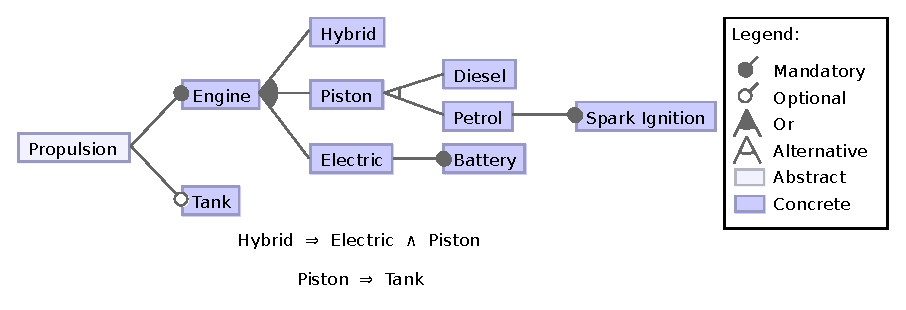
\includegraphics[width=0.85\textwidth]{images/introduction_fm.eps}
  \caption{Feature diagram for a feature model with eight valid configurations;
  two cross-tree constraints are specified as propositional formulas over
  features}
  \label{fig:introduction_fm}
\end{figure}

For a configurable system configurations are primarily chosen to meet
functional and/or non-functional requirements. Nonetheless, the selection of
certain combinations of multiple features, of course, can happen to cause
unexpected and undesired side effects as well. This so-called \emph{feature
interaction} is an ``emergent behavior that cannot be easily deduced from the
behaviors associated with the individual features involved''
\citep{apel_feature-oriented_2013} and can make development and
maintenance of a configurable system an error prone task. 
A commonly referred to example of a feature interaction, as drafted by
\cite{calder_feature_2003}, describes interactions in telecommunication networks. Given two
independent features \textsf{CallForwarding} and \textsf{CallWaiting}, where \textsf{CallForwarding} forwards a call from a busy line to a line that is
available, and where \textsf{CallWaiting} notifies a busy line when a call is on
hold. In isolation their behavior is well-defined, but if both features are selected their oppositional
behavior becomes problematic. If no precedence of one feature has been
specified, the network might end up in race conditions or other unexpected
behavior. That is, to avoid this feature interaction, for instance, precedence
constraints must be implemented or the selection of both features must be
mutually exclusive.


\paragraph*{Thesis Statement and Scope}
A software system’s performance depends on the functionality offered, the
respective implementation, program load and the resulting execution. While
feature interactions not necessarily cause the software system to break
severely in all cases, its overall performance can degrade for corner cases or
specific configurations as the feature selection influences the execution. That
is, the choice of features as well shapes the performance of a software system.

Configuration options for software systems are usually constrained (e.g., are
mutually exclusive, imply or depend on other features) to a certain extent. In
the worst case though, where all options can be selected independently, the
number of valid configurations grows exponentially with every feature added and
likely exceeds the number of atoms in the entire universe once we count $265$
independent features. Hence, even for a small number of features, any naive
approach to assessing properties of configurable software systems exhaustively
for each valid configuration is in general conceived infeasible. Despite this
mathematical limitation, many feasible approaches to static analysis for highly
configurable systems emerged. Those variability-aware approaches enable, for
instance, type checking in the presence of variability by
exploiting commonalities among different variants \citep{thum_classification_2014}.

The aspect of performance of configurable software systems has gained more
attention recently, even though from a practitioners view, according to
\cite{molyneaux_art_2014}, for the most part performance testing is still not
accommodated to an acceptable degree in the development process.
Assessing performance for configurable systems incorporates obtaining knowledge about the performance of
every valid configuration. In the recent past, the a variety of approaches to
model, learn and predict performance behavior for configurable software system
have emerged. The scheme behind these approaches is the conception of
performance modeling as an optimization problem, i.e., to recover and
approximate performance behavior and respective dependencies from the selection
of configuration options.

Genetic algorithms \citep{guo_genetic_2011,sayyad_scalable_2013}  have shown
reasonable results, yet are not able to handle constraints like mutual
exclusion. In 2012 \citeauthor{siegmund_predicting_2012} proposed a
method to predict performance for arbitrary variants following an approach for
automated detection of feature interaction \citep{siegmund_predicting_2012}.
Following their approach, in 2015 they proposed performance-influence models as a means
to analyze and predict performance for configurable software systems
\citep{siegmund_performance-influence_2015}. A performance-influence model
attempts to approximate the influence of both single features and interacting
features on the software systems' performance.
The approach has shown a reasonably low error rate for several real-world
applications and allows prediction of system performance for arbitrary
configuration variants.

Going a step further, actively maintained configurable software systems, of
course, evolve: Variability models might change as software has to adapt to
changes in the functional requirements it is meant to meet. Patching and
upgrading a software system affects the architecture or implementation that is
likely to become inconsistent and degrade over time. While there exists
substantial work on understanding the evolution of configurable systems, e.g.,
documenting common symptoms of architectural decay \citep{passos_feature_2015,zhang_variability_2013} or
attempting to classify patterns for variability evolution
\citep{seidl_co-evolution_2012,peng_analyzing_2011,passos_towards_2012}, there
is little we know so far about the evolution of performance or non-functional
properties in configurable systems.

We believe that to get a better understanding software evolution and to address
performance regression problems it is inevitable to continue studying the
performance and performance evolution of configurable systems. In practice, all
aforementioned approaches to model and predict performance behavior for a
configurable software system require exhaustive records of performance
measurements to learn from. Even though valid configurations can be sampled to
some extent \citep{apel_feature-oriented_2013}, assessing a single version of a configurable software
system still demands a large number of valid configurations to be measured. In
addition, to study the performance evolution of configurable software systems a
history or series of performance models is required. That is, assessing
performance evolution of configurable systems is infeasible without tool
support.\\

The goal of this thesis is to provide a theoretical and practical foundation for
exhaustive performance measurements of configurable software systems and series
thereof. We contribute a guideline of and tool support for performance
measurements in the presence of variable and evolving software. Our research
objectives and desired outcomes are

\begin{itemize}
  \item a survey of the phenomenon of performance evolution and corresponding
  best practices in performance testing, strategies to address configuration space explosion and 
  \item an automated tool support for performance measurement for multiple
  revisions of configurable software systems.
\end{itemize}

\paragraph*{Thesis Outline}
The Thesis is organized as follows. Chapter \ref{chapter:2} recalls the background
topics of the thesis theme, including software evolution, the foundations and statistical
aspects of performance testing, variability model synthesis, and recent
approaches to performance modeling. In Chapter \ref{chapter:3} we present the
overall measurement process and discuss the methods used for our performance
measurement tool as well as its limitations. In Chapter \ref{chapter:4} we evaluate practical
aspects of our tool with respect to practicality and discuss the results
thereof. Finally, Chapter \ref{chapter:5} concludes the thesis and gives an
outlook on possible future work.


\chapter{Background and Related Work}\label{chapter:2}
This chapter presents necessary background to the individual topics used in this
thesis. In section\,\ref{sec:variability_modeling}, we recapitulate
basic concepts, notations, and terminology regarding variability modeling. In
section\,\ref{sec:evolving_solftware}, we outline different aspects of software evolution.
section~\ref{sec:assessing_performance} discusses the assessment and testing of
performance and finally, section\,\ref{sec:performance_prediction_models}
recalls methodology to predict performance behavior for configurable systems. In Section\,\ref{sec:relatedwork} we
review a body of related work that has either touched on topics similar to ours, or pursues a similar methodology, yet with different basic premises.

\section{Variability Modeling} \label{sec:variability_modeling}
The design and development of configurable software systems is conceptually
divided into \emph{problem space} and \emph{solution space} \citep{czarnecki_generative_2000}. The problem space
comprises the abstract design of features that are contained in the software
system as well as constraints defined among features, such as dependencies or mutual exclusion.
The solution space describes the technical realization of features and the
functionality described by and associated with features, e.g., implementation
and build mechanisms. That is, features cross both spaces since they are mapped
to corresponding code artifacts.

A common way to express features and constraints in the problem space is to
define a \emph{variability model}, or \emph{feature model}, which subsumes all
valid configurations
\citep{kang_feature-oriented_1990,thum_reasoning_2009,apel_feature-oriented_2013}.
There are different and equivalent syntactical approaches to define feature
models, for instance, a propositional formula $F$ over the set of features of
the configurable software systems \citep{batory_feature_2005}. In this case, a
configuration is valid with respect to the feature model if and only if $F$
holds for all selected features being true and all unselected features being
false, respectively.
However, a more practical and more commonly used way to express feature models
are graphical tree-like \emph{feature diagrams}
\citep{apel_feature-oriented_2013}. In a feature diagram, features are ordered
hierarchically, starting with a root feature and subsequent child features. By
definition, the selection of a child feature requires the parent feature to be
selected as well. Child features can either be labeled as \emph{optional}
features  or \emph{mandatory} features; the latter ones need to be selected in
every configuration.
Moreover, feature diagrams
provide a syntax for two different types of feature groups, \emph{or-groups} and
\emph{alternative-groups}. For an or-group, at least one of the group's features
needs to be selected for a valid configuration, whereas for an alternative-group
exactly one out of the group's mutually exclusive features must be selected. In
addition to the feature hierarchy, constraints, which cannot be expressed by
the tree-like structure, are referred to as \emph{cross-tree constraints}.
Cross-tree constraints, depending on the notation, are depicted by arrows
between two features or simply added to the feature diagram as a propositional
formula. For two features $f_1$ and $f_2$, a cross-tree constraint means
that for feature $f_1$ to be selected, either the selection of $f_2$ is
required/implied or excluded.

An introductory example for the syntax and semantics of feature diagrams is
provided in Figure~\ref{fig:introduction_fm}. In this example, an imaginary
vehicle propulsion can be configured with eight valid configurations. The
vehicle requires an engine, and therefore feature \textsf{Engine} is mandatory.
At least one out of the three features \textsf{Hybrid}, \textsf{Piston} and 
\textsf{Electric} needs to be selected. For a piston engine, we can select 
either the feature \textsf{Diesel} or \textsf{Petrol}. A petrol engine requires
additional ignition sparks in contrast to a Diesel engine. For an electric
engine, we require a battery, hence, the feature \textsf{Battery} is mandatory.
In addition, the feature model specifies two cross-tree constraints: First, the
feature \textsf{Tank} is optional, yet once a piston engine is selected, we
require  a tank. Second, if we want to use the \textsf{Hybrid} functionality
(e.g., use both electric and piston engine simultaneously), we require to have both a piston
and an electric engine.

\begin{figure}[htbp]
  \centering
  
  	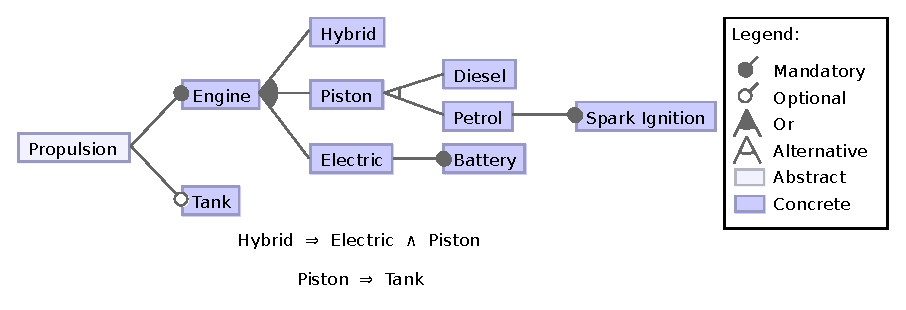
\includegraphics[width=0.85\textwidth]{images/introduction_fm.eps}
  \caption{Feature diagram for a feature model with eight valid configurations;
  two cross-tree constraints are specified as propositional formulas over
  features}
  \label{fig:introduction_fm}
\end{figure}

\section{Software Evolution} \label{sec:evolving_solftware}
The first notion of the software development process is usually
developer-centered and merely focuses on software being designed, implemented,
tested, and eventually being released and deployed.
Maintainability is a generally recognized software quality
property to look after, and maintenance is, of course, essential to every
successful software system \cite{liggesmeyer_software-qualitat:_2009}. Nonetheless, less attention is given to
the ability to adapt a software system to changing requirements (evolvability) rather than maintaining it to keep functionality
working \citep{parnas_software_1994}. Software evolution and evolvability, such
as software itself are manifold. Software evolves in many ways ranging from
maintenance (refactoring, bug-fixes, and patches) to adapting to changed
requirements (adding, removing, reorganizing functionality, and variability).
Modern software systems not only often ship with a variety of configuration
options to select from, they also employ routines to be build and sometimes even
make use of or are part of platforms, such as apps or plugins. That is,
software evolution affects all aforementioned aspects, maintainability as
well as evolvability can degrade as software evolves.

\subsection{Software Erosion}
The negative symptoms of software evolution which are referred to as
``architectural erosion'' \citep{breivold_systematic_2012} have
been addressed by many researchers.
Most of existing research so far though focuses on evolution with regard to
software architecture \citep{breivold_systematic_2012}. The main driving factors leading to symptoms of decay
identified by \cite{perry_software_1991} are architectural erosion and
architectural drift. While architectural drift subsumes developers'
insensitivity when not following a systems architecture or respective guidelines while making changes, architectural erosion subsumes ignoring and violating the existing software
architecture. \cite{parnas_software_1994} argues that as software evolves, software is maintained
and evolved by developers who are not necessarily familiar with the initial
architectural design. Therefore, knowledge about the architecture can become
unavailable as software evolves. Although the unfavorable effects of software
evolution do not break a system necessarily and imminently, the software becomes ``brittle'' \citep{perry_software_1991}
as maintainability as well as evolvability degrade. Concrete  symptoms of software
erosion on the implementation level have been documented. 

\cite{zhang_variability_2013} have studied erosion symptoms for a large-scale
industrial software product line with compile-time variability using
preprocessor directives.
The authors identify variability-related directives and clusters of those that
tend to become more complex as the software evolves. The negative effects, or symptoms of software
erosion are described as, but not limited to \emph{code replication} and
inter-dependencies between code elements, such as \emph{scattering} and
\emph{tangling}. Code scattering describes the phenomenon of code belonging to
a certain feature being scattered across multiple units of implementation,
such as modules, whereas code tangling means that code from different and
potentially unrelated features in entangled within a single module. A figurative
and recapitulative term to refer to the trade-off between postponed maintenance
or QA tasks and the corresponding cost is \emph{technical debt}
\cite{guo_tracking_2011}; the metaphor summarizes the growing risk of quality degradation for eroding software.

\cite{passos_feature_2015} have studied the extent of usage of scattering for device-drivers
in the Linux kernel. Despite scattering being quite prevalent, their
findings suggest that the kernel architecture is robust enough to have evolved
successfully. Nonetheless, platform drivers in the Linux kernel seem more
likely to be scattered than non-platform drivers. They conclude that this is a
trade-off between maintainability and performance: a more generalized and
abstract implementation for platform-drivers in this case could possibly avoid
scattering, yet refactorings in this manner did not seem to be necessary or
worth the effort yet. 


\subsection{Variability Evolution}
Apart from architecture evolution, the variability offered by software systems
evolves as well. For configurable software systems,
evolution steps will not only affect artifacts in the solution space, yet also
be visible in changes in the respective variability models in the problem space.
Although the variability aspect of software evolution has not gathered as
much attention as architecture in the past, more and more
research has emerged recently to address and understand variability evolution.

\cite{peng_analyzing_2011} proposed a classification of variability evolution patterns that
conceives evolution as adaption to changing (non-)functional requirements and
contexts. For a context in that sense, two categories exist. A driving context
determines, whether a variability model and respective variants can meet
functional requirements in the first place. A supporting context by definition
determines how non-functional properties are strengthened or weakened. 
Any changed requirement is likely to change the contexts for a software systems
variability model and, therefore, will make adaptations of the variability
model necessary. Within their classification method, \cite{peng_analyzing_2011} identify major
causes for variability evolution, comprising (a) new driving contexts emerging,
(b) weakened supporting contexts (for instance, due to new non-functional 
requirements), and (c) unfavorable trade-offs for non-functional properties.

To understand single evolutionary steps, several catalogs of variability
evolution patterns have been proposed. \cite{peng_analyzing_2011} present three patterns,
where either a new feature is added, a mandatory feature becomes optional, or a
mandatory/optional feature is split into alternative features. \cite{seidl_co-evolution_2012} suggest a catalog of
patterns for co-evolution of variability models and feature mappings that additionally introduces code clones, splitting a feature
into more fine-grained sub-features, and feature removal as evolution patterns.
In addition, \cite{passos_towards_2012} have studied variability evolution in
the Linux kernel and present a catalog of patterns where features are removed from the
variability model, but remain a part of the implementation. Their
catalog, among others, includes feature merges, either implicit (optional feature merged
with its parent) or explicit.

The classification proposed by \cite{peng_analyzing_2011} is a general and formalized approach
that, as well as \cite{seidl_co-evolution_2012} and \cite{passos_towards_2012}, describes
elementary evolution patterns which can be composed to more complex patterns. Nonetheless, no
comprehensive catalog of variability evolution patterns so far has been
proposed.

\section{Assessing Performance} \label{sec:assessing_performance}
While the last three sections covered software evolution and variability
modeling, we now step forward to the topic of software performance. This
section will outline the term performance with respect to software systems as
well as to possible measurements. We provide a brief look at the general performance
testing setup and the required prerequisites, including suitable benchmarks.
Finally, we provide the statistical background to summarize, interpret and
compare performance measurements accurately.

\subsection{What is Performance?}
The performance of software systems is, like software quality, primarily a
matter of perspective. While an end user might consider practical aspects to be
more important, from a developer’s perspective, performance relates to and is
best described by non-functional properties
\citep{liggesmeyer_software-qualitat:_2009,molyneaux_art_2014}.
While functional properties subsume what exactly a software system does, non-functional
properties describe how (good or bad) a software system is at providing the
functionality offered \citep{liggesmeyer_software-qualitat:_2009}. The notion
of good and bad in this sense corresponds to non-functional requirements (NFR),
that is, software with ``good'' performance behavior does not violate its NFRs.
The categories of NFRs that shape performance behavior are manifold. According to \cite{molyneaux_art_2014}, the categories or
\emph{key performance indicators} (KPIs) include 

\begin{itemize}
  \item availability
  \item response time,
  \item throughput,
  \item resource utilization, and in a broader scope also 
  \item capacity.
\end{itemize}

Time-related KPIs are availability and response time, whereby
availability describes the time or time ratio that the software is available to
the end user, and response time subsumes the time it takes to finish a request
or operation. Throughput as a category subsumes the program behavior with
respect to program load, such as hits per second for a Web application or
amount of data processed per second. Resource utilization describes the extent
to which a software system uses the physical resources (CPU time, memory, and
disk, or cache space) of the host machine. Finally, from a Web-centered
perspective, capacity describes measurements with respect to servers and
networks, such as network utilization  (traffic, transmission rate) and server
utilization, such as resource limitations per application on a host server
\citep{molyneaux_art_2014}.

Consequently, the assessment of performance requires a context or testing
target that corresponds to the assessed system under test (SUT). For instance,
for a simple command-line compression tool, suitable KPIs are response time and
throughput, whereas performance for an online shop Web application is better
outlined by availability and capacity.

\subsection{Performance Testing}
The first step in performance testing, prior to defining relevant KPIs and
metrics, is to specify a system operation or \emph{use case}
\citep{woodside_future_2007} to assess performance for. A typical use case includes a well defined task or
workload to process, expected behavior, outcome, and performance
requirements as previously discussed. For the SUT, however, we require a
version that does compile or, in case it is interpreted, is syntactically
correct \citep{molyneaux_art_2014}. With regard to performance assessments as part of
the development process, a code freeze should be obtained since measurement
results are likely to become meaningless for later versions. In addition to
that,  the machine or setup used for performance measurement should ideally be
as close to the production environment as possible, but at least be documented
to compare different runs \citep{molyneaux_art_2014}.

Finally, one or more benchmarks need to be selected to simulate  the program
load for the respective use case. A benchmark, all in all, needs to be
representative, i.e., should relate to the use case or requirement one
 wants to validate. While benchmarks for file compression usually include
multiple different types of media data (text, sound, pictures) such as the
Canterbury corpus\footnote{The Canterbury corpus can be found
here, \url{http://corpus.canterbury.ac.nz/}.}, Web applications can be exposed
to handling with a number of simulated users at the same time
\citep{molyneaux_art_2014}. Benchmarks have often been standardized within
research and engineering communities to provide comparable performance
measurements. A popular example is the Software Performance Evaluation
Corporation (SPEC), a consortium providing a variety of benchmarks such as the
CPU2000\footnote{The benchmark description can be found at \url{https://www.spec.org/cpu2000/}.} processor benchmark consisting of programs with both floating point and integer operations.
Moreover, benchmarks, in a sense of repeatable program load, can be obtained
from load generation software such as ApacheBench\footnote{Manual page of the
Apache tool \texttt{ab}, \url{http://httpd.apache.org/docs/2.4/en/programs/ab.html}.}
for the Apache Web server or simply by measuring performance for test cases
\citep{heger_automated_2013,nguyen_industrial_2014}.

Performance testing heavily relies on tool support, especially for repeating
test cases and recording measurements. Since the
tool solutions for performance testing vary from domain, scale, and purpose, we
will outline  only the general tool architecture. \cite{molyneaux_art_2014}
describes four primary components for a performance testing setup: a scripting module, a
test management module, a load injector, and an analysis module. A scripting module handles the generation or
repetition of use cases which, for instance, can be recorded prior to the test
for Web applications. A test management module creates and executes a test
session, whose program load is generated by one or more load injectors. A load
injector can provide a benchmark by generating items to process, or can simulate
a number of clients for a server-side application. An analysis module, finally,
collects and summarizes data related to the performance testing target. We present more on
summarizing and comparing recorded results in the
sections\,\ref{sec:statistical_considerations} and~\ref{sec:summarization}.


\section{Performance Prediction
Models}\label{sec:performance_prediction_models} In the previous section, we referred to performance, or in detail, the KPIs, as
possible testing targets, which we validate against non-functional requirements.
However, in a broader sense, software performance has become an aspect of
software engineering referred to as \emph{software performance engineering}
(SPE) \citep{woodside_future_2007}.
A lot of effort has been spent to study and describe performance behavior as well
as to improve performance quality. Besides the analysis of concerns or
requirements with respect to performance, SPE comprises performance testing as
well as performance prediction \citep{woodside_future_2007}. Performance
prediction aims at modeling and estimating performance behavior for different
use cases or configurations. The first approaches to performance prediction
models describe the underlying software system component or operation from which
performance estimations are then deduced. These so-called \emph{model-based prediction models} enable a performance estimation early in the development process since no actual
performance measurement is required \citep{woodside_future_2007}. In contrast
to model-based approaches, measurement-based approaches have emerged. These \emph{measurement-based prediction models} are based on a sample of performance
measures which are used to learn a software system's performance behavior
\citep{woodside_future_2007}. More recently, measurement-based prediction models that emphasize variability have been
proposed, of which we will discuss three approaches in the remainder of
this section.

\paragraph{Learning Performance} In essence, learning and predicting
performance behavior for a configurable system means nothing different than finding an
approximation $\hat{f}$ for a function $f: C \rightarrow \mathbb{R}$ where $C$
is the set of configurations and $f(c) \in \mathbb{R}$ with $c \in C$ is the corresponding performance measurement. The
accuracy of the approximation $\hat{f}$ describes how the estimated performance
$\hat{f}(c)$ deviates from the actually measured performance $f(c)$. 
Different approaches to construct such an approximation, referred to as a
\emph{performance prediction model}, emerged recently. All approaches utilize
two samples of configurations and corresponding performance
measurements to build and validate the model. A training sample is used to
learn the approximation from, whereas a testing sample is used to assess the
prediction error rate of the previously learned approximation. 
%While the
%approaches mentioned below differ in the expression of a performance prediction
%model, all require ``meaningful'' training samples and stress the importance of
%sampling strategies.

A straightforward methodology to learn performance behavior was proposed by
\citep{guo_variability-aware_2013}.
The authors utilize classification-and-regression-trees (CART), akin to decision trees, to derive a top-down classification hierarchy for a
given sample. The approach supports progressive (and random) sampling, i.e.,
the performance model is constructed several times while the size of the
training sample is successively increased. The CART is constructed by
recursively partitioning the sample into smaller segments which best describe a
class. It is worth mentioning that the estimation using CART is not limited to
binary configuration options, but supports numeric features as well. Moreover,
the approach by \citep{guo_variability-aware_2013} does not produce any further
computation overhead besides the measurement effort and the construction of a CART.

A different approach to modeling performance behavior was
proposed by \cite{zhang_performance_2015}. The authors propose an approach to construct
performance prediction models based on a Fourier description of the
performance-describing function $f$, which maps each configuration to a
corresponding performance measurement. The principal idea is to approximate a
Fourier series approximating the function  $f$, and
learning all coefficients of the Forier series terms.

The number of terms is exponential in the number of configuration options. The main
characteristic of this approach is that, prior to learning a performance
prediction model, a desired level of prediction accuracy can be specified. That
is, the approach automatically chooses the sample size required to learn the
prediction model accordingly.

A third approach to model and predict performance behavior,
\emph{SPLConqueror}, was proposed by \cite{siegmund_predicting_2012}. The
authors describe performance behavior  for a configuration as the accumulated influence of
features, from which the configuration is composed, and respective feature
interactions. To estimate the influence of single features and feature
interactions, the authors propose a number of sampling strategies. Single
features are assessed by comparing the performance of two different
configurations per feature: For a feature $f$, two valid configurations are
compared, whereby both configurations have the minimal number of features
selected that are not excluded by the selection of $f$. While for one
configuration $f$ is selected, it is deselected for the other one. The
difference between the performance measures for both configurations is the estimate
$\Delta_{min(f)}$ for the performance influence of feature $f$. Feature
interactions that are performance-relevant are detected automatically in a similar manner. The
main idea is, that a feature $f$ is more likely to interact with other features,
the more features are selected along with $f$. Therefore, if $f$ interacts, the
influence of feature $f$,  $\Delta_{min(f)}$ differs from the influence of $f$,
when estimated using configurations where the maximal number of features selectable
together with $f$ are used. Based on the set of interacting features, three
heuristics are employed to detect feature interactions. Simple feature
interactions are detected using pair-wise sampling
\citep{siegmund_predicting_2012,apel_feature-oriented_2013}, whereas
higher-order feature interactions are often composed from simpler ones, or centered
around a small subset of hot-spot features \citep{siegmund_predicting_2012}.
Finally, for an arbitrary configuration, the performance can be predicted by the
sum of influence estimations per feature and feature interaction.

The idea of predicting performance by estimating the influence of feature
and feature interactions was further developed by \cite{siegmund_performance-influence_2015} by
proposing performance-influence models for both binary and numeric
configuration options. A performance influence, similar to \emph{SPLConqueror},
predicts performance by computing the sum of previously learned influence
estimates. The novelty of this approach lies in the way the terms describing
the influence of feature and feature interactions are learned and not
derived from a sampling strategy.
Instead of a single constant performance influence estimate, each term can contain of a
number of functions, such as linear, quadratic, or logarithm functions, or
compositions thereof. This does not only allow the developer to incorporate
domain knowledge by preselecting functions. Moreover, but also by introducing
combinations of non-linear functions and learning the coefficients using linear
regressions, it enables learning a non-linear function. The algorithm commences
with the selection of terms and successively extends and reduces the term selection to increase 
the prediction accuracy. The outcome, similar to
\cite{siegmund_predicting_2012}, is a linear function whose terms represent the estimated influence of features and
feature interactions on performance.

All aforementioned approaches rely on performance measurements and, to
some extent, also on a  sampling strategy. While the approaches by
\cite{siegmund_predicting_2012,siegmund_performance-influence_2015} essentially describe sampling strategies,
the approach proposed by \cite{zhang_performance_2015} is able to work with random samples, and the
approach of \cite{guo_variability-aware_2013} allows a smaller sample to be
extended progressively \citep{guo_variability-aware_2013}.
As performance measurements entails an expensive and time-consuming process,
\cite{sarkar_cost-efficient_2015} have investigated different sampling
strategies in this domain.
The authors compare progressive sampling, where sample sizes are increased
successively until the learned prediction model performs accurately enough, and projective
sampling, where the optimal sample size is estimated based on the expected
learning curve, with respect to cost and prediction accuracy. They advocate the
use of projective sampling over progressive sampling. In addition, the authors
propose and evaluate an own sampling heuristic to select an initial sample for
progressive sampling. This sampling heuristic is based on feature frequencies
and outperforms t-wise sampling, such as pair-wise sampling
\citep{sarkar_cost-efficient_2015}.

\section{Related Work}\label{sec:relatedwork}
While to the best of our knowledge, there exists no previous work on
exhaustively presenting a methodology to understand and comprehend performance
evolution of configurable software system, there is a body of work that has
either touched on similar topics, or pursues a similar methodology, yet with
different basic premises. In the following, we present and summarize related
work to emphasize thelimited scope of our work, and to give an outline of
possible future research directions. Further note that we describe here only
additional approaches to the ones we have already discussed in the previous
sections.

\paragraph{Visualization of Software Evolution.}
Throughout our methodology, we have frequently used diverse visualizations of
data obtained from repository mining, for instance, for commit activity, and as
a basis for revision sampling strategies. In addition, we have taken into
account similar data in the interpretation of our performance evolution history
data in section. Therefore, as software evolves it is inevitable to not
consider those data to obtain more complete and integrated insights.
Aggregation and visualization of aforementioned data records can help to sketch
and understand possible coherences.

\cite{german_visualizing_2006} have presented a comprehensive tool,
\emph{softChange}, to visualize multiple aspects of a software system’s
evolution history, including commit and file activity graphs, authorship
overviews, and visualizations of file coupling. While their tool is not
designed with regard to a specific research direction, the authors stress the
importance of means to aggregate and analyze software trails in order to
explore and understand software evolution. Joint visualizations
of software trails as well as performance evolution history data is a promising
augmentation in the comprehension of multi-layered software evolution.

\cite{wu_exploring_2004} have presented presented an integrated approach to
visualize multiple different measurements over time. Their proposed
\emph{evolution spectrum graphs} are inspired by spectrum visualizations for
audio signals. A spectrum in their context can, for instance,  be a list of files, for which
different measurements are illustrated over time. While this approach allows
for a global overview over an arbitrary timespan, it also can sketch
fine-grained changes and trends over time. Although, according to the authors, the
visualizations need to be tailored to the target system with respect to
coloring and spectrum selection, evolution spectrum graphs can be a useful
means to aggregate and visualize various single-valued measurements for a
spectrum of variants for configurable software systems.

To conclude with a broader overview on visualization tools for further reading,
\cite{storey_use_2005} have surveyed twelve tools (including the previously
mentioned two) that intend to visualize any kind of human activities in
software development with a string focus on software evolution. The authors
evaluate the different tools with respect to different aspects, including
intent of the tools, the information sources utilized by the tools, the form of
presentation offered by the tools, and the effectiveness in terms of
feasibility and validity.

We see these lines of work orthogonal to our methodology such that we can
incorporate different visualization techniques when it comes to evaluating and
understanding the performance evolution of configurable software systems.

\paragraph{Power Consumption Evolution}
\cite{hindle_green_2015} have proposed a methodology, \emph{green mining}, to
measure and model the evolution of power consumption across different versions of a
software system. Using their methodology, the authors have documented the power
consumption evolution history of two different software systems, and identified
feasible metrics to summarize power consumption. 

Compared to our proposed methodology, green mining considers only 
one-dimensional evolution of power consumption as different software variants
are not taken into account, yet green mining examines the relationship between
power consumption and further quality attributes. That is, we believe that
interpreting performance evolution results in an extended context of software
metrics with respect to software architecture, power consumption, and along
established software analyses should direct further research activities towards
a better understanding of software evolution.

\chapter{Methodology: Variability Assessment}\label{sec:chapter:3}
{
\color{blue}
Articles to look into:
\begin{itemize}
  \item \cite{kastner_model_2009}
  \item \cite{apel_semistructured_2011}
  \item \cite{kastner_variability-aware_2011}
  \item \cite{nadi_mining_2014}
  \item \cite{nguyen_building_2014}
  \item \cite{meinicke_essential_2016}
  \item \cite{medeiros_discipline_2017}
\end{itemize}
}

\section{Variability Model Synthesis}  \label{sec:feature_model_synthesis}
A variability model as an abstraction of functionality of a software system is
required, or at least of great interest, in many contexts. 

\emph{First}, not
every configurable system provides an explicit
representation of its variability model. 
The reasons for inexplicit or absent configuration specification are manifold.
They can range from poor or inconsistent documentation
\citep{rabkin_static_2011} to overly complex configurability
\citep{xu_hey_2015}, or configuration constraints originated in different layers of a software
system, such as build constraints  or compiler constraints
\citep{nadi_where_2015}.

\emph{Second}, variability models have emerged to be a useful means in domain
analysis prior to developing a software system. As feature diagrams group and
organize features (representing functionality), synthesizing a variability model
has shown to be applicable to extract features and constraints from functional requirements.
In addition, by comparison of product specifications for an
existing market domain, variability models can provide a detailed feature
summary \citep{alves_exploratory_2008,bakar_feature_2015}.

For this thesis, we focus on the first aspect of synthesizing variability
models as our work addresses the assessment of already existing configurable
software systems. Nonetheless, many techniques employed in the aforementioned
second aspect consider similar problems, yet rely on natural language artifacts
rather than code artifacts \citep{alves_exploratory_2008,bakar_feature_2015}.
The following section recalls work on extracting configuration options and
constraints from source code as well as the organization of constraints into
feature hierarchy and groups. The further assessment of configurable systems
requires a well-defined and sound variability model.

\subsection{Feature Extraction} 
The first objective in recovering a variability model from a configurable
system is to determine the available configuration options to select
from. In addition, for further configuration, the type of each configuration
option (e.g., boolean, numeric, or string) and the respective domain of valid
values needs to be specified.

\cite{rabkin_static_2011} proposed a static, yet heuristic approach to extract
configuration options along with respective types and domains. Their approach
exploits the usage of configuration APIs and works
in two stages. It commences with extracting all code sections where
configuration options are parsed. Next, configuration names can be
recovered as they are either already specified at compile-time or can be
reconstructed using string analysis yielding respective regular expressions.
Moreover, the authors employ a number of heuristics to infer the type of parsed
configurations as well as respective domains. First, the return type of the
parsing method is likely to indicate the type of the configuration option read.
Second, if a string is read initially, the library method it is passed to can
reveal valuable information about the actual type. For instance, a method
\emph{parseInteger} is likely to parse an integer value. Third, whenever a
parsed configuration option is compared against a constant, expression, or value
of an enum class, these might indicate valid values or at least corner cases of
the configuration option domain. The extraction method by
\cite{rabkin_static_2011} is precise, but limited, for instance, when an
option leaves the scope of the source code.
Nonetheless, for the systems studied, the authors were able to recover
configuration options that were not documented, only used for debugging or even not used at
all.

\subsection{Constraint Extraction}
The second step in recovering a variability model is the
extraction of configuration constraints. An approach proposed by \cite{zhou_extracting_2015}
focuses on the extraction of file presence conditions from build files using symbolic execution. A more comprehensive investigation of configuration
constraints and their origin is provided by \cite{nadi_mining_2014,nadi_where_2015}. They
use variability-aware parsing to infer constraints by
evaluating make files and  analyzing preprocessor directives. Inferred
constraints result from violations of two assumed rules, where (a) every valid
configuration must not contain build-time errors and (b) every valid
configuration should result in a lexically different program. While the
first rule aims at inferring constraints that prevent build-time errors, the
second one is intended to detect features without any effect, at least as part
of some configurations. Their analysis one the one hand emerged to be accurate
in recovering constraints with 93\,\% for constraints inferred by the first rule
and 77\,\% for second one respectively. On the other hand, their approach
recovered only 28\,\% of all constraints present in the software system.
Further qualitative investigation, including developer interviews, lead to
the conclusion that most of existing constraints stem from domain knowledge
\citep{nadi_where_2015}.

\subsection{Feature Hierarchy Recovery} \label{sec:feature_hierarchy}
Besides recovering configuration options and respective constraints, to reverse
engineer a feature model, one further step is required. The recovered knowledge
needs to be organized in a tree-like hierarchy with feature groups specified and
CTCs explicitly stated to derive a valid feature diagram 
\citep{kang_feature-oriented_1990}.
While several approaches for recovering the feature model hierarchy have been
proposed, we are primarily interested in finding a hierarchy for knowledge
obtained from source code. Other scenarios, as already stated in the opener of
this section, are based on product descriptions or sets of valid configurations
\citep{aleti_software_2013,bakar_feature_2015}. In the remainder of this
subsection, we will focus on organizing features and constraints extracted from
source code. For further reading, \cite{andersen_efficient_2012} present algorithms for structuring feature diagrams for three different scenarios including the ones previously mentioned.

Given an extracted set of features along with corresponding descriptions and
recovered constraints among the features, \cite{she_reverse_2011} propose a
semi-automated and interactive approach to synthesize a feature hierarchy.
Their approach comprises three tasks. First, an overall feature hierarchy based
on feature implications is specified. Second, potential feature groups are
detected and manually selected. Finally, the feature diagram is extended with
remaining CTCs. A detailed description of the algorithm is presented below:

\begin{enumerate}
  \item The algorithm commences with finding a single parent for each
  feature and, thus, specifying a tree-like feature hierarchy. Based on the
  given constraints, a directed acyclic graph (DAG) representing implication
  relationships among features, a so-called \emph{implication graph}, is
  constructed.
  Every vertex in the implication graph represents a feature  and edges are
  inserted for each pair of features $(u, v)$, where  $u \implies v$ holds with respect to the given
  constraints.
   
  In addition to the implication graph, the algorithm for each feature computes
  two rankings of features that are likely to be the respective parent feature.
  The two rankings both employ the feature descriptions. Feature descriptions
  are compared for similarity using a similarity metric. For two features $p$
  and $s$, the similarity is defined as the weighted sum of the inverse document
  frequencies $idf(w)$ for the words that both descriptions of features $p$
  and $s$ share.
  The $idf$-ranking for a word $w$ is the logarithm of the number of features
  divided by the number of features whose description contains $w$. Each $idf$
  value is weighted with the frequency of $w$ in the description of
  feature $p$.
  
  The first ranking, called Ranked-Implied-Features (RIF), for each feature $f$
  ranks all features by their similarity to $f$ in an descending order, but
  prioritizes those features that are implied according to the previously
  computed implication graph. The second ranking, called Ranked-All-Features
  (RAF) is similar to RIF, yet less strict since implied features are not
  prioritized. Given these rankings, a user for each feature selects a suitable
  parent feature from the RIF or RAF ranking. The idea behind providing two
  separate rankings, according to \cite{she_reverse_2011} is that the given
  extracted constraints can be incomplete and, thus, not all relevant
  implications are contained in the implication graph.

  \item After the feature hierarchy is specified, another auxiliary graph, a
  mutex graph, similar to the implication graph, is constructed. The \emph{mutex
  graph} is an undirected graph with features as vertices and edges between two
  features $u$ and $v$, if $u \implies \neg{v}$ and $v \implies \neg{u}$ hold
  with respect to the given constraints. 
  That is, all adjacent features are mutually exclusive. Based on
  this mutex graph, all maximal cliques (subsets of vertices that all are
  connected with each other) among the vertices with the same parent are
  computed. All features within such a clique are mutually exclusive and share
  the same parent and represent mutex- or alternative-groups. \cite{she_reverse_2011} introduce an
  additional constraint to extract xor-groups that require one of the groups’
  features to be selected if the parent is selected. This distinction is in
  line with the initial description of feature diagrams by \cite{kang_feature-oriented_1990},
  but not all descriptions of feature diagrams follow this distinction between
  mutex- and xor-groups and just use the term alternative-group discussed in 
  Sec. \ref{sec:variability_modeling}. %2.1
  
  \item CTCs for the feature diagram are extracted from
  the given configuration constraints. Since CTCs are constraints that could
  not be represented by the feature hierarchy (implication) or
  alternative-groups (exclusion), the derivation of CTCs follows this idea. The
  set of cross-tree implications is derived by removing all edges that are part
  of the feature hierarchy from the initially constructed implication graph.
  The set of cross-tree exclusions is derived similarly from the mutex
  graph by removing all edges among vertices of all mutex-groups. To make the
  feature model sound, the given configuration constraints, reduced to those
  clauses that are not already entailed by the diagram, can be added as an
  additional CTC formula to the feature diagram \citep{she_reverse_2011}.
\end{enumerate}

The approach by \cite{she_reverse_2011} provides a practical algorithm to synthesize a
feature diagram, yet has some limitations we need to consider. First, the
approach is not able to detect or-groups as defined in Sec. \ref{sec:variability_modeling}.
Second, the approach does introduce a root feature. Finally, the approach does not
distinguish between mandatory and optional features. Implicitly, all features
that do not have a parent feature are optional and all features that have a
parent feature are by default mandatory. \cite{she_reverse_2011} evaluated the
algorithm with both complete and incomplete variability knowledge (feature
names, descriptions and constraints). While the algorithm has shown to be
practical, detecting features whose parent was the root-feature was difficult
since, due to the transitive property of implication, it is implied by each
feature of the feature model.

\subsection{Variability Model Synthesis in Practice}
\begin{itemize}
  \item How do the previously mentioned approaches relate to real-world
  situations?
  \item What artifacts can be used aside from code?
\end{itemize}

\section{Configuration Generation}
Apart from having knowledge about the variability of a configurable software
system, either in the form of a set of constraints among features, or a feature
diagram, we also need to derive all configurations, but at least meaningful
sample sets thereof, from the variability model. Variability models can be
expressed in various forms, such as propositional formulas or context-free
grammars (CFG) \citep{batory_feature_2005}, as well as constraint satisfaction
problems (CSP) \citep{benavides_automated_2005,benavides_using_2005}.
Accordingly, the all configurations represent solutions to propositional formulas or CSPs, and valid words for CFGs
respectively. That is, the generation of all configurations with respect to the
variability model is equivalent to finding a solution or word set for the
aforementioned representations of a variability model. In the following, we
look into how variability models can be encoded as a CSP and describe in detail
the configuration generation using CFGs.

\subsection{Constraint Satisfaction Problem}
A constraint satisfaction problem (CSP) in the context of variability modeling
describes a set of options ranging over finite domain as well as a set of
constraints which restrict which values variables can take simultaneously
\citep{benavides_automated_2005}. Fo a binary option $b$, the respective domain
$dom(b)$ simply is $\lbrace 0, 1\rbrace$.
For a numeric option, the respective domain $dom(n)$ is a finite set of legal
values with a minimum and a maximum value, say $\lbrace v_{min}, v_1,
v_2, \ldots, v_{max}\rbrace$.
A solution $s: O \rightarrow dom(o_1) \times dom(o_2) \times \ldots \times
dom(o_{|O|})$ to a CSP is an assignment of options $o_i \in O, i \in \mathbb{N}$
to values of their respective domain, such that all constraints are satisfied simultaneously \citep{benavides_automated_2005}.  

A solution to a CSP is found by systematically checking for different
selections of values whether all constraints are satisfied. There exists a
large number of ready-to-use SAT and CSP solvers, yet we are not covering CSP
solution here since it is beyond the scope of your thesis. For further reading, 
\citep{benavides_fama:_2007} present a tool with extensive analysis support for
various different presentations of variability models.

To encode a variability model as a CSP, \cite{benavides_automated_2005} describe
the following transformation rules:

\begin{itemize}
  \item For a parent feature $f$ and a child feature $f’$, a mandatory
  relationship is expressed as $f \Leftrightarrow f’$, and an optional relationship is
  expressed as $f’ \implies f$.
    \item  For a parent feature $f$ and child features $f_i$, where $i = 1, 2,
    \ldots n$, an or-group is expressed as $f \Leftrightarrow f_1 \lor f_2 \lor
    \ldots \lor f_n$, and an alternative-group is expressed as $$\bigwedge_{i
    = 0}^n f_i \Leftrightarrow (f \land \bigwedge_{j \in \lbrack 0, n \rbrack
    \setminus i} \neg f_j) $$.
\end{itemize}

To also consider numeric options, the domain of a numeric option $n$ can be
conceived as an alternative-group since only one value from the domain can be
selected at a time. Hence, each value of the domain $dom(n)$ can be conceived as
a binary option. If value $v \in dom(n)$ is selected, this states $n = v$,
otherwise $n \neq v$.


\subsection{Grammar Expansion}
Besides trying to find solution for satisfiability problems, the expression of
variability models as context-free grammars (CFGs) enables the derivation of
configurations directly from a CFG by expanding it. A
first description of transformation rules, yet only for feature diagrams with
binary options, was was proposed by \cite{batory_feature_2005}. A hierarchical feature diagram
can be recovered from a set of constraints using the algorithm of
\cite{she_reverse_2011} as explained in section \ref{sec:feature_hierarchy}.
In the following we describe
how a feature diagram with both binary and numeric features can be transformed
to a context-free grammar, and how configurations can be derived subsequently.

\begin{definition}[Context-free Grammar]\label{def:cfg}
A context-free grammar is a tuple $G = (N, T, S, P)$, consisting of a set of
non-terminal symbols $N$, a set of terminal symbols $T$, a start word $S \in (N
\cup T)^*$, and a set of productions $P \subseteq N \times (N \cup T)^*$. The
set $L_G$ describes the language of the grammar $G$ and comprises all valid
words $w \in L_G$ which can be derived from the start word $S \in L_G$ by
applying productions a finite number of times to it.
\end{definition}

Following the Definition.~\ref{def:cfg}, to derive all configurations for a
given feature diagram, the idea is to first translate it to a context-free
grammar. In order to do so, especially with respect to handling numeric
options, we introduce an extended definition for a CFG, a configuration
generation grammar.

\begin{definition}[Configuration Generation Grammar]\label{def:cgg}
A configuration generation grammar is a context-free grammar $G = (N, T, S,
P)$ whose elements are constructed from a feature diagram as follows.

\begin{itemize}
  \item All features represent non-terminal symbols $N$, which can be divided
  into two disjoint sets, binary non-terminal symbols $F_\mathcal{B}$ and
  numeric nont-terminal symbols $F_\mathcal{N}$. That is, $N = F_\mathcal{B}
  \cup F_\mathcal{N}$ and $F_\mathcal{B} \cap F_\mathcal{N} = \varnothing$.

  \item Similarly, the set of terminal symbols $T$ is consists of two different
  sets, the binary terminal symbols $T_\mathcal{B}$ and the numeric terminal
  symbols $T_\mathcal{N}$, so that $T = T_\mathcal{B} \cup T_\mathcal{N}$ and
  $T_\mathcal{B} \cap T_\mathcal{N} = \varnothing$ with
  
  \begin{equation}
  T_\mathcal{B} = \bigcup_{b\in F_\mathcal{B}} \lbrace b_0,  b_1\rbrace
  \end{equation}
  
  \begin{equation}
  T_\mathcal{N} = \bigcup_{n\in F_\mathcal{N}} ~ \bigcup_{v_i \in dom(n)}
  \lbrace n_{v_i}\rbrace.
  \end{equation}
  
  \item All productions $P$ are constructed from the hierarchy specified in the
  given feature diagram, the binary, and the numeric features. In our definition
  of a configuration grammar, each word $w$ is expressed as a subset of
  (non-)terminal symbols, i.e., $w \subseteq (N \cup T)$. A word is a terminal
  word, if and only if it does not contain any non-terminal symbol. Accordingly,
  the set of productions is $P \subseteq N \times (N \cup T)$, and a production
  $p = (u, v) \in P$ is applied to a word $w$ by removing non-terminal symbol
  $u$ from word $w$ and merging words $v$ and $w$. Hence, the new word $w'$ is
  defined as $w' = (w \setminus u) \cup v$.

  The productions $P = P_H \cup P_F$ are constructed from the following disjoint
  two sets of productions:
  
  \begin{equation}
  P_H = \lbrace (p, \lbrace c, c_1 \rbrace) | p, c \in N \land
  c \implies p\rbrace
  \end{equation}
  
  \begin{equation}
  P_F = \bigcup_{f \in (F_\mathcal{B} \cup F_\mathcal{N})} ~ \bigcup_{v \in
  dom(f)} \lbrace (f, v) \rbrace
  \end{equation}
	
  \item Finally, the start word $S \subseteq (N \cup T)$ consists the
  non-terminal representing the top-level feature in the given feature diagram.
  The set of respective configurations is described by all words which can be
  generated by a finite number of applications of productions to the start word
  $S$.
  
  \end{itemize}
\end{definition}

Based on definition \ref{def:cgg}, we specify the following algorithm
\ref{alg:expand} to expand the configuration step by step and, thus, derive all valid words from the
grammar. The algorithm repeatedly derives new words by applying every production
possible to previously derived words. Once a word is terminal, i.e., does not
contain any non-terminal symbol, it is returned and not expanded any further.
The algorithm terminates if there is no word left to expand in the queue of
partial words.\\

\begin{algorithm}[H]\label{alg:expand}
 \KwData{Configuration generation grammar $G = \lbrace N, T, S, P \rbrace$, and
 cross-tree constraints $C$ of the given variability model}
 \KwResult{All configurations of the given variability model.}
 \vspace{5mm}
 words = Queue()\;
 words.enqueue($S$)\;
 \While{words is not empty}{
  current = words.dequeue()\;
  \If{current does violate any cross-tree constraint}{
   continue\;
   }
   \For{$n \in N$}{
   		\If{$n \in current$}{
   			\For{$u \in \lbrace u | (n, u) \in P \rbrace$}{
   				new = current\;
   				new = new $\setminus~ n$\;
   				new = new $\cup~ u$\;
   				\eIf{$N \cup new = \varnothing$}{
   					yield new\;
   				}{
   					words.enqueue(new)\;
   				}
   			}
   			break\;
   		}
   }
 }
 
 \caption{Expansion algorithm for a configuration generation grammar.}
\end{algorithm}\vspace{2mm}

In addition to deriving all configurations from a variability model, the
algorithm can also be used to derive partial configurations, such as
binary-only configurations. To do so, the numeric features need to be removed
from the set of non-terminal symbols. The only limitation of this algorithm is
that, conceptually, it requires all numeric options to be mandatory features.
This is due to the unspecified semantics of a numeric option being un- or
deselected.

\section{Configuration Sampling}
\begin{itemize}
  \item Sampling strategies with respect to coverage criteria
  \citep{apel_feature-oriented_2013}
  \item Evaluation of different sampling strategies \citep{medeiros_comparison_2016}
  \item Influence-centered sampling \cite{siegmund_predicting_2012}
\end{itemize}

\subsection{Sampling for Binary Features}
\subsection{Sampling for Numeric Features}


\chapter{Methodology: Version Assessment}\label{chapter:4}
In the last chapter, we have covered means to understand variability,
synthesize variability models for a given software system, and to select sample
sets of configurations. To enable the assessment of performance evolution for
configurable software systems, the next step in our methodology takes into
account the dimension of diachrony. As software evolves, multiple versions, or
called revisions, of a software system exist. In this chapter, we address the
question of how we can assess performance for multiple revisions. Moreover, we
ask whether we can describe a configurable software systems’ performance
evolution without exhaustively assessing all versions by selecting only a
sample set of versions. As illustrated in the methodological road-map in
Figure~\ref{fig:roadmap_2}, we summarize these two questions with the task of
revision sampling.

\begin{figure}[h!]
	\centering
	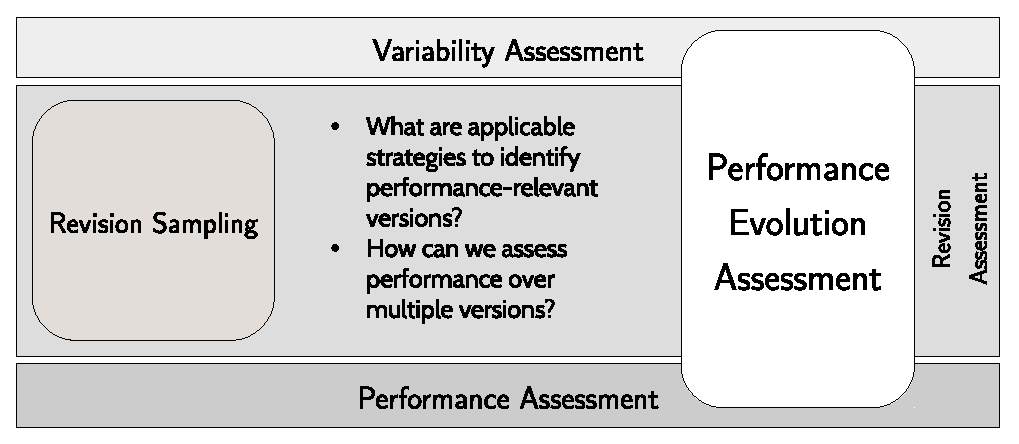
\includegraphics[width=0.75\textwidth]{images/process_revassesment.eps}
	\caption{Methodological road-map: questions to address with revision
	assessment.}
	\label{fig:roadmap_2}
\end{figure}

The chapter is organized as follows. In section~\ref{sec:towards_revsampling} we
present the methodological requirements for a designing and selecting a revision sampling
strategy. In section ~\ref{sec:revsampling_strat} we propose five approaches to
revision sampling based on observations of configurable software systems. In
section~\ref{sec:revsampling_eval} we evaluate the different approaches against
exhaustive measurements of a selection of configurable software systems.
Finally, in section~\ref{sec:revsampling_method} we conclude the chapter and
discuss the approaches' applicability in the context of our methodology.

\section{Towards Revision Sampling}\label{sec:towards_revsampling}
Research so far has addressed the assessment of a software system’s revision
history under the umbrella of repository mining, for instance, to localize bugs
\citep{moin_bug_2010} or performance regression \citep{heger_automated_2013}.
Nonetheless, so far there exists little to no research addressing the question
what the choice of versions might reveal about performance evolution. The task
of selecting resources and a sample set of versions to analyze can be conceived
as a sampling strategy, where the objective is to cover interesting entities
(performance changes, in our case) while trying to limit the sample size to
keep the required effort reasonable. Before we present different approaches to
select a sample set of revisions, we need to define general cornerstones for
evaluating a sample set of revisions as well as respective revision sampling
strategies with respect to performance change history.

\paragraph{Revision Sample Set.} The first question is, what criteria we take as
a basis for rating a sample set of revisions as \emph{meaningful}. First, our intention
is to obtain a representative description of a software system’s performance
change history while only assessing a fraction of revisions. That is, assessing
a representative sample of revisions should yield a performance change history
similar to the assessment of all revisions. Since we are interested in
revisions for which performance measurements change, these revisions should be
contained in a representative sample. Second, especially in the context of
variability, a performance change might only affect a subset of the assessed
configurations. A representative sample set, therefore, should describe a
history of significant performance changes with respect to all variants
assessed. We consider a performance change to be significant, if it affects a
significant portion of the sample of variants (effect range) and if the
relative change in performance measurements is significantly huge (effect
magnitude).

\begin{figure}[h!]
	\centering
	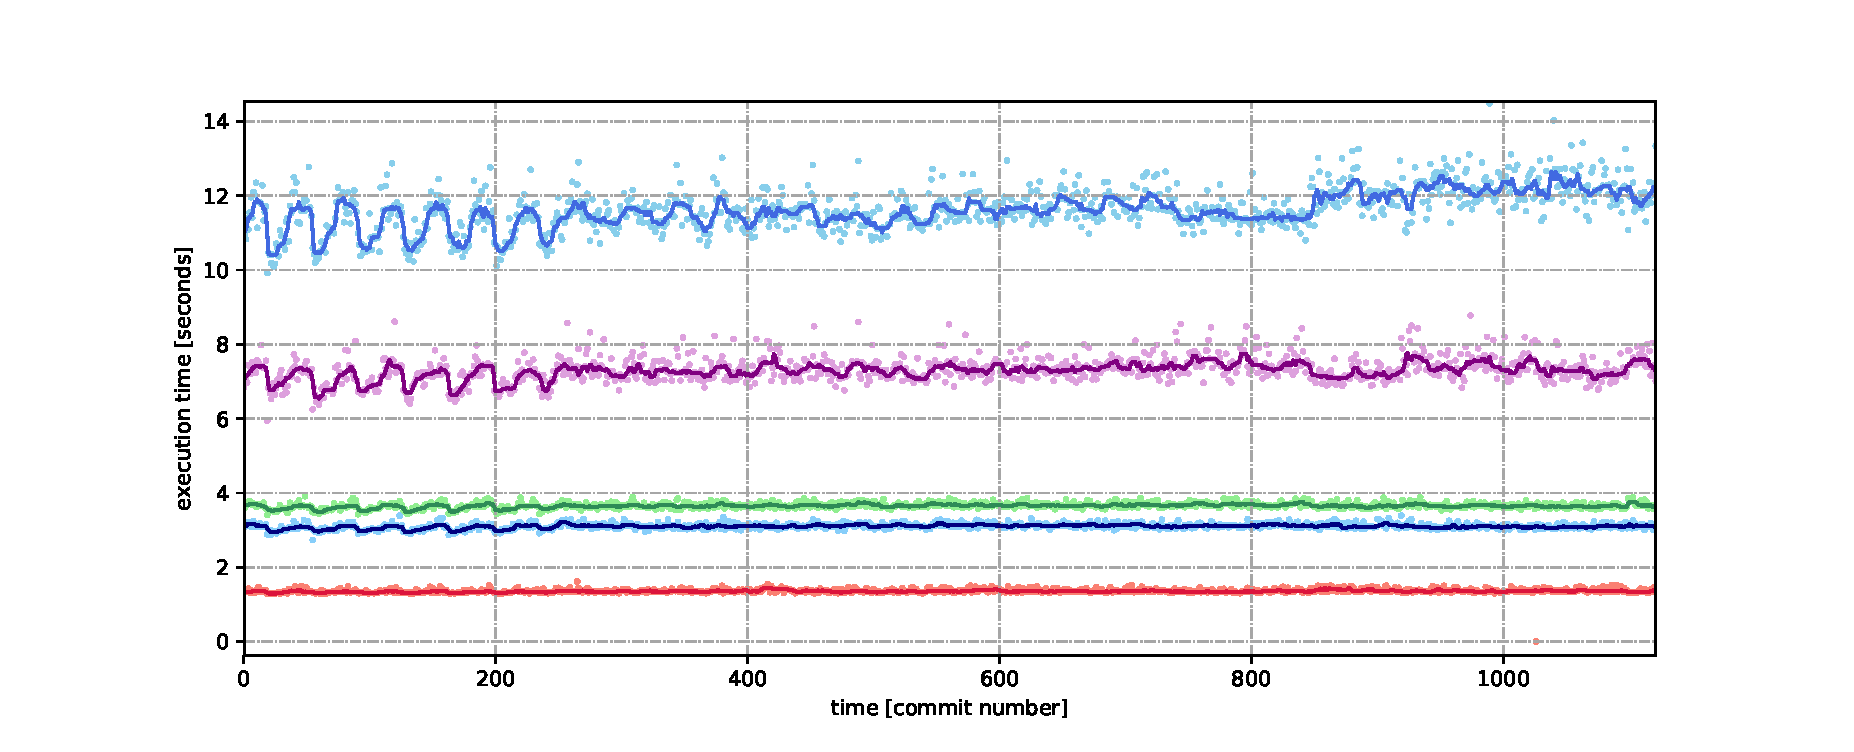
\includegraphics[width=0.95\textwidth]{images/xz_sample_evolution.eps}
	\caption{Performance History for XZ}
	\label{fig:xz_evosample}
\end{figure}

To illustrate the two facets of performance changes, in
Figure~\ref{fig:xz_evosample} we see a history of performance measurements (execution time in this case) for a
small-scale configurable software system, file compression tool called \emph{GNU
XZ Utils}. The graphic depicts execution time measures for executing a standard
compression benchmark for $1,135$ different versions and covers a version
history of about nine years. In this excerpt, we only show the execution time measures
of four different variants, i.e., each version was assessed with four different
configurations. One can see that the execution time for the red and the green
configurations remains stable and does not fluctuate, while for the blue and
grey configuration, the execution time measures are generally more volatile.
Moreover, between 2010 and 2012, performance for the latter variants fluctuates
heavily. With regard to the two facets of significance mentioned above, not all
variants are affected similarly by this effect. That is, if performance were
assessed solely for one of the non-fluctuating variants, no performance
evolution could be identified.

While the former significance criterion can unambiguously defined by a threshold
number of variants, for the latter one one needs to define how to summarize
relative performance change among all variants. For instance, a performance
change may have a significant magnitude, if the average deviation of
performance measurements for all variants is greater than a specified threshold
value.

\paragraph{Revision Sampling Strategies.} The second question addresses the
rationale behind a revision sampling strategy. To obtain representative sample sets, sampling
strategies are intended to utilize knowledge about the total volume to select
sample sets from. For instance, pair-wise sampling aims to cover most feature
interactions. Similarly, we demand for a meaningful revision sampling strategy
to exhibit a certain rationale or coverage criterion. If we conceive a sampling
strategy as a binary classificator that, in our case, decides whether in a
revision a performance change is likely, or performance measurements might have
changed compared to prior commits, we want  this classifier to be sensitive,
i.e., to have a preferably high true positive rate. That is, a sampling
strategy is meaningful if we learn which revision features most likely indicate
performance evolution.
 
\section{Revision Sampling Strategies}\label{sec:revsampling_strat}

\begin{figure}[h!]
\centering
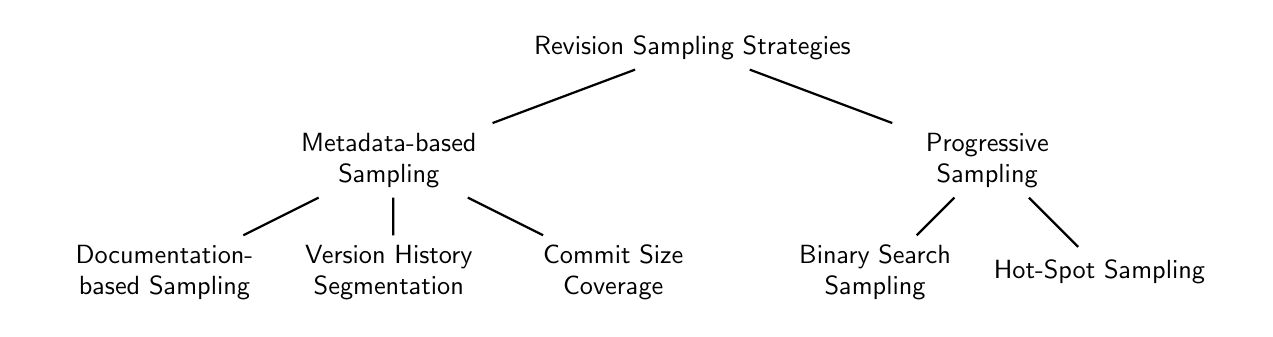
\begin{tikzpicture}[%sibling distance=15em,
level 1/.style={sibling distance=8cm},
level 2/.style={sibling distance=3cm}, 
level 3/.style={sibling distance=6cm},
  every node/.style = {rounded corners,
    draw, align=center,
    top color=white, bottom color=blue!20},thick,scale=0.95, every
    node/.style={scale=0.95}]
  \node {\sffamily Revision Sampling Strategies}
    child { 
    	node [align=left] {
    		\begin{tabular}{c} 
    			{\sffamily \parbox{3cm}{\centering Metadata-based Sampling}}
    		\end{tabular}
    	}
    	child { 
    		node [align=left] {
    			\begin{tabular}{c}
    				{\sffamily \parbox{3cm}{\centering Documentation-based Sampling}}
    			\end{tabular}
    		}
    	} 
    	child { 
    		node [align=left] {
    			\begin{tabular}{c} 
    				{\sffamily \parbox{3cm}{\centering Version History Segmentation}}
    			\end{tabular}
    		}
    	}
    	child { 
    		node [align=left] {
    			\begin{tabular}{c} 
    				{\sffamily \parbox{3cm}{\centering Commit Size Coverage}}
    			\end{tabular}
    		}
    	} 
    }
    child { 
    	node [align=left] {
    		\begin{tabular}{c} 
    			{\sffamily \parbox{3cm}{\centering Progressive Sampling}}
    		\end{tabular}
    	} 
    	child { 
    		node [align=left] {
    			\begin{tabular}{c}
    				{\sffamily \parbox{3cm}{\centering Binary Search Sampling}}
    			\end{tabular}
    		}
    	} 
    	child { 
    		node [align=left] {
	    		\begin{tabular}{c} 
	    			{\sffamily \parbox{3cm}{\centering Hot-Spot Sampling}}
	    		\end{tabular}
    		}
    	} 
    };
\end{tikzpicture}
\caption{Overview of our proposed revision
sampling strategies.}\label{fig:revsampling_overview}
\end{figure}

\subsection{Documentation-driven Sampling}
\subsection{Version History Segmentation}
\subsection{Change Coverage Sampling}
\subsection{Binary-Search-based Sampling}
\subsection{Hot-Spot Sampling}

\section{Strategy Evaluation}\label{sec:revsampling_eval}
\section{Methodological Remarks}\label{sec:revsampling_method}

%\begin{figure}
%\def\tabularxcolumn#1{m{#1}}
%\begin{tabularx}{\linewidth}{@{}cXX@{}}
%\begin{tabular}{c}
%\subfloat[Activity Graph for \texttt{GNU XZ}, generated from 399 versions
%between March 24, 2017, and August 14, 2017. The earliest release version is
%\texttt{5.1.1alpha}, the latest is \texttt{5.3.0alpha}.]
%{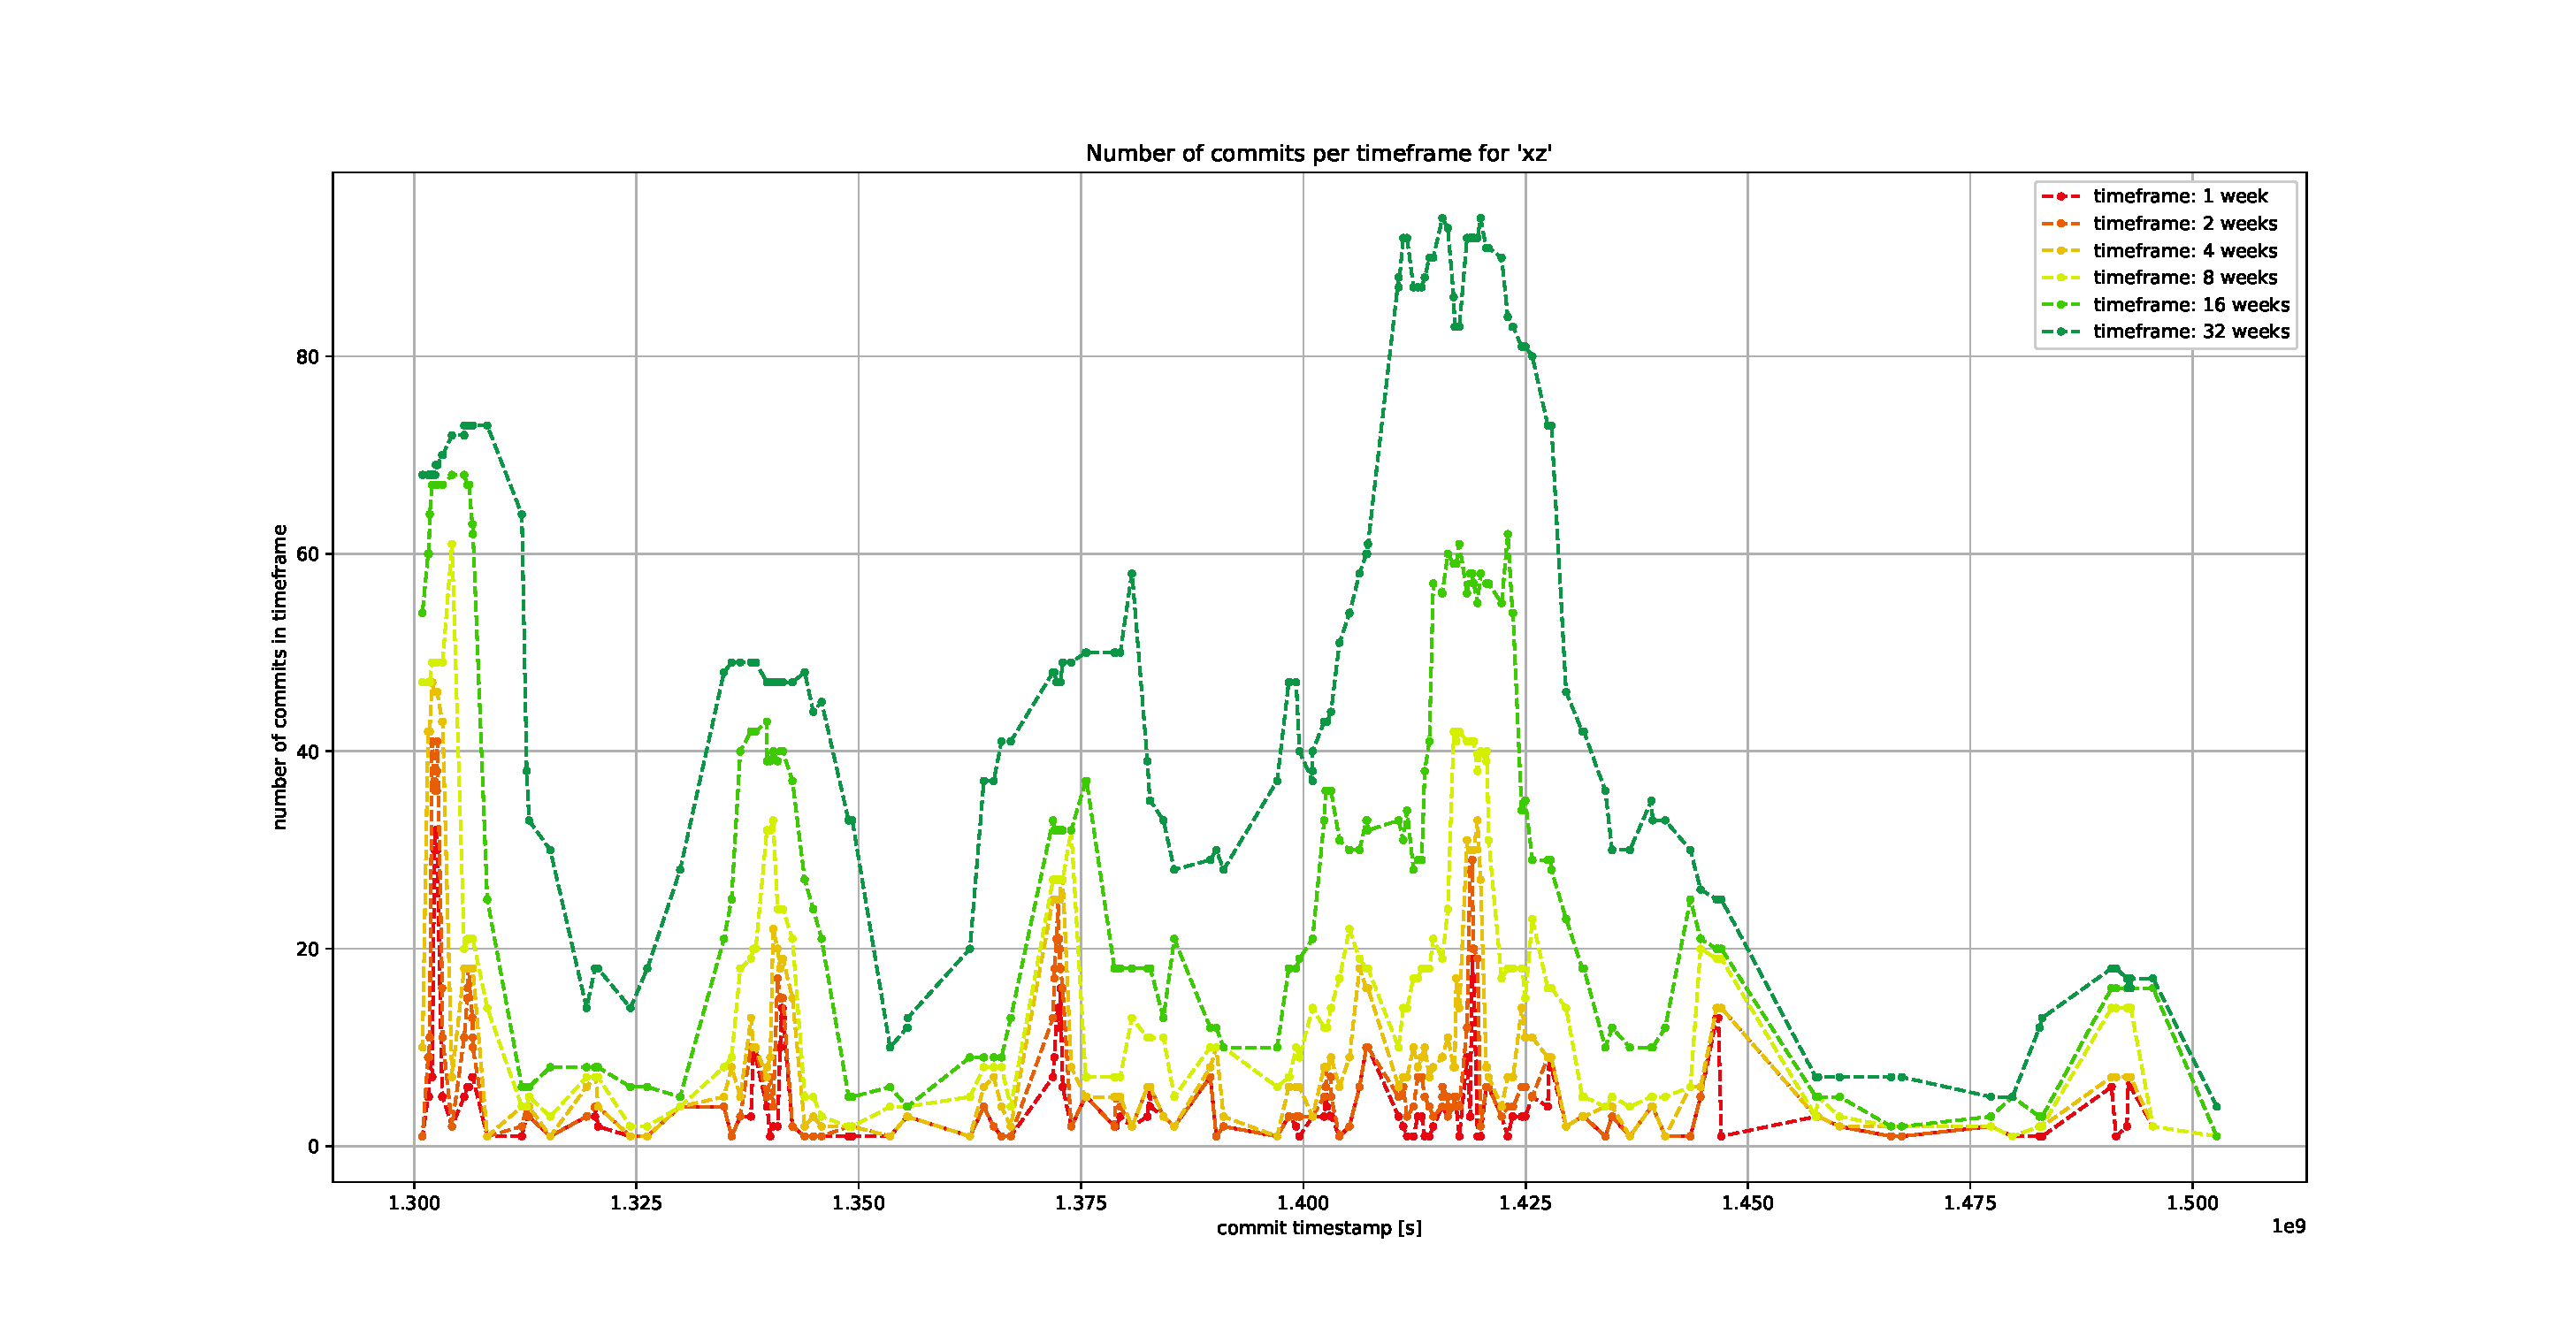
\includegraphics[width=0.99\textwidth]{images/activity_xz.eps}}
%\\
%\subfloat[Activity Graph for \texttt{x264}, generated from 2851 versions
%between June 3, 2004, and June 26, 2017. The earliest release version is
%\texttt{BUILD 1} from, the latest is \texttt{BUILD 149} from
%X.]{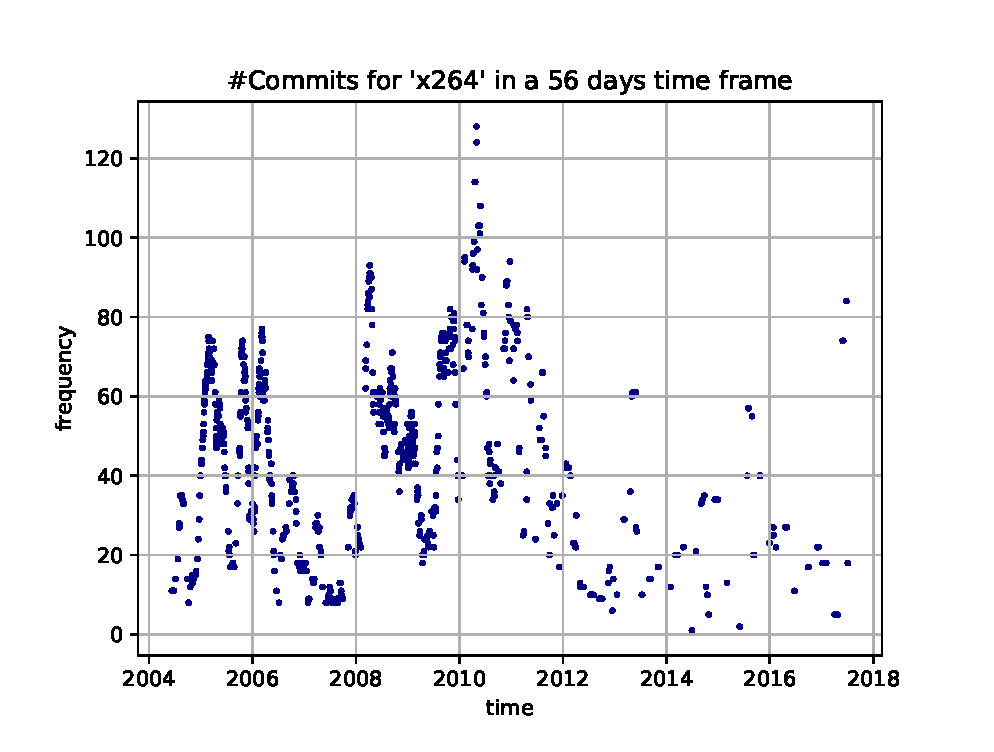
\includegraphics[width=0.99\textwidth]{images/activity_x264.eps}}\\
%\end{tabular}
%\end{tabularx}
%\caption{Commit activity for two sample systems, the compression
%utility \texttt{GNU XZ} and the video encoder \texttt{x264}. For each version,
%the activity is measured as the number of commits that were pushed within a
%certain timeframe after or before the actual commit. The timeframes range from
%one week to 32 weeks, as shown in the legendary.}
%\label{fig:ActivityGraphs}
%\end{figure}


\chapter{Methodology: Performance Assessment}\label{chapter:5}
The last two chapters covered methodological guidelines for variability as well
as version assessment. While those two terms, \emph{variability} and
\emph{versions} represent two orthogonal dimensions of a configurable software
systems’ evolution history. To provide a closed description of guidelines for performance
evolution assessment, this chapter finally presents a guideline to assessing
performance for a given variant and version. In Figure~\ref{fig:roadmap_3}, we
present the methodological roadmap and questions to be answered in this chapter.

\begin{figure}[h!]
	\centering
	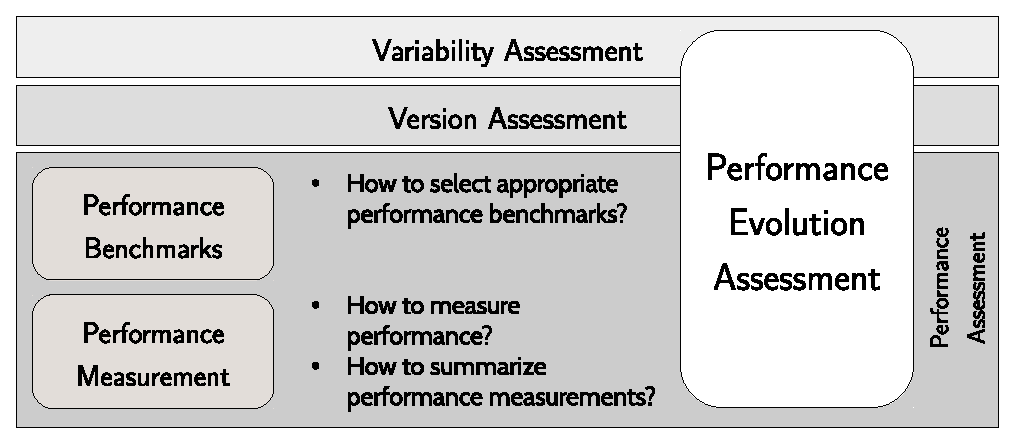
\includegraphics[width=0.9\textwidth]{images/process_perfassessment.eps}
	\caption{Methodological road-map: performance assessment}
	\label{fig:roadmap_3}
\end{figure}

First, in section we categorize software systems with respect to the availability of suitable performance
benchmarks; second, we outline the general properties of profiling tool support
used throughout dynamic program analysis; finally, we discuss different statistical
with respect to their applicability in the context of performance assessment
and robustness.

\section{Performance Benchmarks}
The essential part of assessing performance for a software system is the choice
of a benchmark that one wants to evaluate the software against. For the choice
of a suitable benchmark, two consecutive questions need to be answered. First of
all, we need to specify, what aspects of performance we intend to evaluate for
our software system. As presented earlier in chapter 2, the term performance is
generic as it is commonly outlined by different key performance indicators. For
instance, for a web shop application, good performance is characterized by low response
time and high availability, while for file compression, one might rather
conceive high throughput as good performance. That is, given a specific
aspect of performance, i.e., one or more KPIs, for a software system, from
testing against a suitable performance benchmark one needs to be able to judge
whether the specified performance goals are met, or not.

Next, once we have specified performance indicators fitting our software system,
we need to select a benchmark, i.e., a repeatable task for the software system
for which we can evaluate performance. To keep performance measurements
comparable throughout all versions and variants, it is required to use
only one benchmark per assessment. Following this principle, and to even compare different software
systems, practitioners are advised to refer to reusable, or more general
performance benchmarks whenever possible. To illustrate this, we can divide
software systems into three general categories for which we are presenting
separate strategies.

First, in the the easiest case, a software system provides software tests, or
performance benchmarks, to use for performance assessment. The idea of using an
existing test suite to assess performance is straightforward and has already
been applied to detect performance regression
\citep{foo_mining_2010,heger_automated_2013}.

Second, a software system can offer functionality for a domain, where
standardized benchmarks have been established, or are commonly used to compare
performance measurements. For instance, for the domain of file compression
there exists a long tradition of using standardized file sets as performance
benchmarks, such as the Canterbury
or Calgary corpus\footnote{See
\url{http://corpus.canterbury.ac.nz/descriptions/} for a detailed 
description.}; for video encoding, the
xiph.org\footnote{\url{https://media.xiph.org/}} foundation provides a large set of video benchmark files; and, more general, for processors the Standard
Performance Evaluation Corporation provides (SPEC) standardized benchmarks for
floating point operations. Whenever a software system falls under a domain for
which standardized benchmarks exist, we advocate to use those.

Finally, if neither a performance benchmark or test suite is available for a
software system, nor domain-specific benchmarks exist, the task of designing a
benchmark is left to the practitioner evaluating the software. As the
conception of performance is generic and highly context-dependent, there is no
standardized recipe for designing a performance benchmark. However, the main
criteria to be satisfied include \emph{expressiveness}, \emph{cost-efficiency}
and \emph{reproducibility}. First, a suitable performance benchmark should
clearly express what a desirable and unfavorable performance measurement is, given a specified
key performance indicator. For instance, if we evaluate performance in terms of
response, or execution time, minimal measurements are desirable. Second, effort
that is required to evaluate a software with a benchmark must be reasonable.
Since performance measurements are usually repeated to decrease measurement
bias, or used for different variants and revisions, performance benchmarks
should be limited in terms of size. However, a performance benchmark needs to
be large enough to sketch performance changes or deviations. Finally, the
construction of a benchmark must be reproducible, i.e., transparent and
plausibly designed as the overall value of a performance benchmark depends on
whether we can draw any conclusion from performance measurements obtained from
it.

In conclusion, for the context of our methodology, the advocated guideline for
selecting and designing a performance benchmark for a configurable software
system is to select a benchmark as generic as possible. If there is no reusable
benchmark available, the design of any performance benchmark should follow the
criteria of expressiveness, cost-efficiency, and reproducibility.

\section{Profiling}
With a software system along with a benchmark set up, the only choice left
before assessing performance is to select a means to obtain and collect
performance measurements. For this type of tool support for dynamic analysis,
commonly referred to as profilers, exists a variety of solutions, varying in
functionality and scope of application.

\cite{satapathy_survey_2015} have surveyed a selection of profilers for dynamic
analysis. The authors categorize their selection into three categories,
including VM-profiling-based, instumentation-based, and profilers based on
aspect-oriented programming (AOP). While for VM-based profilers, make use of
profiling functionality offered by the respective platform, such as the Common
Language Interface (CLI) for the family of .NET languages,  or the Java Virtual
Machine (JVM), instrumentation-based profilers add instructions to the software
to the software’s codebase at compilation using instrumentation preprocessors,
or to the software’s executables. AOP-based profilers accommodate profiling
functionality in separate modules called aspects. An aspect’s code, called
advise is executed whenever a corresponding event, called join point,  occurs,
for instance a call of a function that one would like to measure performance
for. Several join points can be summarized by a set of join points, called
point cut. While VM-based profilers are limited to a family of programming
languages, and, as well as instrumentation-based, usually introduce a run-time
overhead that might dilute performance measurements. In contrast to that,
AOP-based profilers  usually perform better, yet are limited to the code base as aspects
are woven into the codebase during re-compilation. Moreover, they require a
higher level of expertise to design and deploy a performance test setup
compared to the former two categories \citep{satapathy_survey_2015}. In addition
to the aforementioned profiler categories, statistical profilers such as
\emph{Performance Counters for
Linux}\footnote{See
\url{http://man7.org/linux/man-pages/man1/perf-stat.1.html} for further
information on \texttt{perf}.}, or \emph{perf}, monitor a software system
performance, for instance hardware counters for regular intervals, and therefore provide an approximation of the software system’s performance with less overhead than instrumentation-based profilers.

In the context of our methodology, we are advocating the use of the unix
command \texttt{time}\footnote{See
\url{http://man7.org/linux/man-pages/man1/time.1.html} for the man page of
\texttt{time} and provided performance metrics to record.} to measure execution
time along with a number of further performance metrics for a software system.
The command is contained in most Linux distributions and, from a black-box
perspective, provides sufficient functionality to sketch performance in terms of
metrics for execution time, memory consumption, or I/O statistics. While tools falling under the aforementioned categories are powerful tools for dynamic analysis and program
optimization, time provides a basic, yet exhaustive support for assessing
performance for software system run on a single host machine. 

\section{Statistical Considerations}\label{sec:statistical_considerations}
In this section, we now discuss the appropriate statistical means to summarize,
compare and interpret measurement results. For the remainder of this section, we
will refer to the following two scenarios. First, to obtain robust results, the
assessment of a single variant needs to be repeated multiple times.
Consequently, to report a single result per metric, the measurements for a
single variant need to be summarized. Second, the assessment of performance for
a variant may comprise several use cases, for instance file
compression and decompression for a compression software. Therefore, performance measures
aggregated from different benchmarks need to be summarized accurately. 

\subsection{Measures of Central Tendency}
For each test run of a software system or variant, we obtain a single-valued
measurement per performance metric. Since we repeat each test run $n$ times
per variant, we obtain a data record $X$ with $n$ measurements $X = X_1, X_2,
\ldots, X_{n-1}, X_n$. While the arithmetic mean is commonly considered the
right way to summarize data records and report a representative average
value, we need to be more cautious with how to summarize data records
\citep{fleming_how_1986,smith_characterizing_1988}. From a statistical
perspective, the intention of summarizing a data record is to find a measure of
central tendency what is representative for the data record.
While the arithmetic mean is an appropriate method for many cases, there exist
other means to summarize data records. Moreover, there exist a number of
criteria for when to use which means to summarize a data record. 

The first question when summarizing a data
record is to ask what the data actually describe and what we intend to express
with our summary. For a data record $X$, we can define a
relationship we would like to conserve while replacing each single $X_i$ with an
average value $\bar{x}$. Based on this relationship, we can derive the
appropriate method to summarize our record. For instance, our data record $X$
describes the time elapsed for a test case and we want the keep the following
relation, saying that the sum of all measurements $\sum_{i = 1}^{n} X_i$ is
equal to the total time elapsed $T$, defined as

$$
T = \sum_{i = 1}^{n} X_i = \sum_{i = 1}^{n} \bar{x}.
$$

Based on the term above, we can derive the definition of the method
appropriate to summarize our data record with respect to the conserved relation
what is the \emph{arithmetic mean}, defined as

\begin{equation} \label{eq:arithmetic_mean}
\begin{split}
\bar{x} = \frac{1}{n} \sum_{i = 1}^{n} X_i.
\end{split}
\end{equation}

Consider another example, similar to the one above, where the test
case is a load test with a predefined number of users and the measurements $X =
X_1, X_2, \ldots, X_{n-1}, X_n$ are
measured as hits per second. Again, we have different measurements we want to
summarize with respect to a relation to conserve. Each user drops the same
number of requests $T$, whereby the hit rate $X_i$ and the respective elapsed
time $t_i = \frac{T}{X_i }$ vary. We now conserve the relationship that the
total number of requests for the data record is the sum of all hit rates $X_i$
times the time elapsed $t_i$. Therefore, we want to substitute each hit rate
$X_i$ with an average value $\hat{x}$ so that the aforementioned relationship is
conserved:

$$
n\cdot T - \sum_{n}^{i=1} X_it_i = 0 \Leftrightarrow n\cdot T - \hat{v}
\sum_{n}^{i=1} t_i = 0 \Leftrightarrow n = \hat{x} \sum_{n}^{i=1} \frac{1}{X_i}
$$

Similar to Eq. \ref{eq:arithmetic_mean} we can derive the definition for the summarization
method to use from the equation above what is the \emph{harmonic mean}, defined as

\begin{equation} \label{eq:harmonic_mean}
\begin{split}
\hat{x} = n \cdot \bigg(\sum_{i=1}^{n} \frac{1}{X_i}\bigg)^{-1} =
\frac{n}{\frac{1}{X_1} + \frac{1}{X_2} + \ldots +
\frac{1}{X_{n-1}} + \frac{1}{X_n}}.
\end{split}
\end{equation}

We see that the summarization methods presented in Eq. \ref{eq:arithmetic_mean}
and \ref{eq:harmonic_mean} are useful for different types of data records, and
should be used accordingly. The arithmetic mean is suitable for records, where the total sum of single
measurements has a meaning, whereas the harmonic mean is suitable for measured
rates or frequencies \citep{smith_characterizing_1988}.

While the aforementioned measures of central tendency should be appropriate for
most cases, they are not always the best choice though since the arithmetic
and harmonic mean are heavily influenced by extreme observations
\citep{shanmugam_statistics_2015}. 
For instance, for the data record $X = 1, 2, 3, 30$, three of four values are
smaller than the arithmetic mean $\bar{x} = 9$. One option is to explicitly exclude outlier
values from the data record. The so-called \emph{trimmed mean} is
obtained by truncating a upper and/or lower percentage $t$ of the data record
and, consequently, computing the (arithmetic or harmonic) mean for the remaining
data record \citep{shanmugam_statistics_2015}. 

While this method is suitable to omit the effects of outliers, one still needs to specify
which upper and/or lower percentage $t$ needs to be truncated. Moreover, the use
a (trimmed) mean requires the data records' frequencies to be distributed
symmetrically around its mean.
A probability distribution is skewed (and therefore asymmetric) if, graphically speaking, its histogram is not
symmetric around its measure of central tendency. A simple method to measure the
skewness of a probability distribution is \emph{Bowley's measure}
\citep{shanmugam_statistics_2015}, defined as

\begin{equation} \label{eq:bowley}
\begin{split}
B_S = \frac{(Q_3 - M) - (M - Q_1)}{Q_3 - Q_1} = \frac{(Q_3 + Q_1 - 2M)}{Q_3
- Q_1},
\end{split}
\end{equation}

where $Q_1$ and $Q_3$ denote the first and third quartile, and $M$ denotes the
median of the probability distribution. The quartiles $Q_i$ with $i \in \left\{
1,2,3 \right\}$ are defined as the values of a data record $X$, so that
$\frac{i}{4}$ of the values of $X$ are smaller than $Q_i$. The \emph{median} is
defined as $Q_2$, i.e., a value $M \in X$ so that half of the values in $X$ are smaller than $M$.

The median itself is a more robust measure of central tendency than the
aforementioned ones since it is less influenced by outliers and can be used for
both skewed and symmetric data records \citep{shanmugam_statistics_2015}. For a
given ascendingly ordered data record $X = X_1, X_2, \ldots, X_{n-1}, X_n$, we
can compute the median as follows:

\begin{equation} \label{eq:median}
\mathrm{Median}(X) = \begin{cases}
     X_{\frac{n+1}{2}} & \text{if $n$ is odd} \\
     \frac{1}{2}\big(X_{\frac{n}{2}} + X_{\frac{n}{2}+1}\big) & \text{if $n$ is
     even}
   \end{cases}~\text{with $X_i \leq X_j$ and $i < j \leq n$ }
\end{equation}

\subsection{Measures of Dispersion}

Last, we take a look at different measures of spread or dispersion. Most
commonly used are the \emph{variance} $\sigma^2$ and the \emph{standard
deviation} $\sigma = \sqrt{\sigma^2}$ defined along the mean $\mu$ of a
probability distribution as

\begin{equation} \label{eq:variance}
\begin{split}
\sigma^2 = \frac{\sum_{i=1}^{n}(X_i - \mu)^2}{n}
\end{split}
\end{equation}

Similar to the (arithmetic or harmonic) mean, the variance and the standard
deviation are heavily influenced by extreme observations
\citep{shanmugam_statistics_2015} and not the best choice in all cases. Instead,
two more robust measures are the \emph{median absolute deviation} (MAD) and the \emph{inter-quartile range} (IQR). The MAD is defined as the median of the absolute deviations from the probability distributions'
median \citep{molyneaux_art_2014}, or, defined as follows:

\begin{equation} \label{eq:mad}
\begin{split}
\mathrm{MAD}(X) = \mathrm{Median}\big(|X - \mathrm{Median}(X)|\big)
\end{split}
\end{equation}
 
The IQR, however, defines the range between the first and the third quartile,
$Q_1$ and $Q_3$ \citep{shanmugam_statistics_2015}. This range is larger for a
widespread data record and smaller for a data range with a narrow spread, but is not influenced by extreme
observations as those outliers do not lie within the range $\left[ Q_1,Q_3
\right] $. The IQR is defined as 

\begin{equation} \label{eq:iqr}
\begin{split}
\mathrm{IQR}(X) = Q_3 - Q_1.
\end{split}
\end{equation}

\subsection{When to use which measure?}
In this section we discussed the arithmetic and harmonic mean as well as the
median as a measure of central tendency, the symmetric property that is
required to use the arithmetic or harmonic mean, and different measures of
spread for a given data record. At the beginning, we have raised the question of how to
summarize data records (a) for an experiment repeated multiple times, and (b)
obtained from different benchmarks. While for case (b) the answer is to use the
arithmetic or harmonic mean (depending on the quality of the measurements), for
(a) the answer is a little more elaborate.

The arithmetic (or harmonic) mean can be used whenever the quality of the
measurement is appropriate and the data record is symmetric. According to
\cite{shanmugam_statistics_2015}, the arithmetic mean is preferable ``when the numbers combine
additively to produce a resultant value'', such as time periods or memory sizes, whereas
the harmonic mean is preferable ``when reciprocals of several non-zero numbers
combine additively to produce a resultant value'', such as rates or frequencies
\citep{smith_characterizing_1988}.
The median is a less precise estimator than the both means, yet more robust
with regard to extreme observations. In addition, the MAD or IQR provide a more
robust means of spread than the standard deviation.

\section{Summarization Strategies}
Besides the statistical considerations regarding the summarization of
performance measurements, we are also challenged by the dimensionality of our
performance evolution history. Given a record of performance measurements for a
number of versions across different variants, we require statistical and
numerical means to summarize performance evolution with single values. For this
purpose, we propose two metrics addressing the following two aspects. First,
different variants usually exhibit different levels of performance
measurements, aside from evolution and fluctuations. To effectively compare the
performance change of different variants, we propose to use the relative
performance change as a suitable metric. Second, performance changes do not
necessarily affect all variants in a similar way. To measure the homogeneity of
perfornance changes across different variants, we propose to use the variance
of changes per version. A mathematical definition for both relative performance
change and performance change variance is given below.

\subsection{Relative Performance Change}\label{sec:relativechange}
Let $P$ be a $M \times N$ matrix with performance measurements $p_{i, j}$ with
$i, j \in \mathbb{N}, i \leq M, j \leq N$ for $M$ versions and $N$ variants. Now
we compute the relative performance change as a $M \times N$ matrix $P'$ as
follows:

\begin{equation}
   p'_{i, j} =
   \begin{cases}
     0 & \text{if~} i = 1 \\
     \frac{p_{i, j}}{p_{i-1,j}} - 1 & \text{else} 
   \end{cases}
\end{equation}

The relative performance change provides a normalized means to compare
performance changes for different variants of a configurabel software systems.

\subsection{Performance Change Variance}\label{sec:changevar}
Let $P'$ be a $M \times N$ matrix with relative performance change measurements.
To measure the homogeneity of performance changes across different variants, we
compute $v_i$ the variance all variants' relative performance changes for a
version $i$ with $i \leq M$ as follows:

\begin{equation}
   v_i = \text{Var}\lbrace p'_{i,1},\,p'_{i,2},\,\ldots,\,p'_{i,N-1},\,p'_{i,N}
   \rbrace
\end{equation}

The variance increases the more the relative performance changes spread, i.e.
the more heterogeneously different variants evolve.


\chapter{Evaluation} \label{chapter:6}
In the last three chapters, we have presented our methodology to assess the
performance evolution history of configurable software systems. The first part
covered a catalog of methods to derive a variability model from the software
system or related resources along with different strategies to select sample
sets of variants. In the second part, we presented and evaluated different
strategies to select a subset of revisions, for which performance measurements
approximate the overall performance evolution history. The third part reviewed
aspects on concrete performance measurement, including guidelines to follow when choosing
a benchmark to test, and when summarizing measurement results across different
variants and versions.

While the evaluation of revision sampling strategies in the previous chapter
already presented some performance measurement results ex ante, in this chapter, we
evaluate the applicability of our methodology with a case study. With our case
study we intend to answer the following research questions:

\begin{enumerate}[RQ1)]
  \item \emph{Does the methodlogy meet its objectives?}
  \item \emph{Does performance evolve?}
  \item \emph{Does our methodology accurately describe performance evolution?}
  \item \emph{Are our performance measurements reliable?}
\end{enumerate}

{\color{red}This chapter is organized as follows. In section 6.1 we present our
case study corpus, i.e., the selection of configurable software systems that we
assess performance for in our experiment. Section 6.1 addresses RQ1 by
documenting how we followed our methodology throughout the experiment setup and
conduction. Section 6.2 addresses RQ2  with an extensive description of
performance evolution results and insights obtained from it. Finally, section
6.3 addresses RQ3 and RQ4 by reviewing the accuracy of revision sampling
strategies and assessing the reliability of our performance measurement
approach.
}

\section{Case Study Corpus}\label{sec:casestudy}
To evaluate our methodology, we selected two subject systems: GNU XZ and
x264. The selection process accounted for the following requirements. First,
since our intention is to assess the performance evolution history of a
configurable software system, we limited our selection to mature software
systems that exhibit a development history of a couple years or more. Second,
we limit our selection to software systems for which we can obtain a
fine-grained development history, usually version control logs. The rational is that our methodology considers the sampling of different revisions as
well as the possibility to manually inquire possible causes of performance
changes. Third, we intend to consider software systems that have already been
subject of related research, such as work on performance prediction models.
This enables us to compare our results with, and place our results in the
context of previous work. Lastly, the scope of this case study is constrained
by limited time. Hence, the selection of software systems to assess is not
representative, yet intended to validate the methodology presented earlier, and
to obtain empirical insights on whether, and if so, how performance evolves for
configurable software systems.

Our case study corpus comprises two configurable software systems, GNU
XZ\footnote{Find the project description of GNU XZ at
\url{https://tukaani.org/xz/}.} and x264\footnote{Find the project description
of x264 at \url{https://www.videolan.org/developers/x264.html}}.
GNU XZ is a free file compression tool that is widely used across the open-source universe. GNU XZ provides a development history of about ten years,
or more than 1,100 versions,  and is actively maintained as part of the GNU
project. It provides a publicly accessible Git repository as well as additional
resources, such as archived mailing lists and bug reports. The software itself
has not been subject of related research, yet it has been frequently compared
with other file compression tools with respect to compression performance. 

x264 is a free library implementation of the H.264 codec for video encoding,
commonly known as MPEG-4. The implementation provides a command line interface
to use and has been subject of previous research, including performance
prediction models
\citep{siegmund_predicting_2012,siegmund_performance-influence_2015}. Similar to
GNU XZ, x264 is a mature software system that provides a development history of almost ten years, or more than 2,800 versions. Both software systems are configurable at load-time
via command line arguments that modify the file compression process, or video
encoding process, respectively.

\section{RQ1: Does the methodology meet its objectives?}\label{sec:expsetup}
In the following, we document the application of our methodology to the two
software systems of our case study corpus. In particular, this section covers
the aspects of variability- and performance assessment since we have already
covered the results for revision sampling in chapter 4. 

All performance measurements made in the
following were conducted on a Linux machine (Debian 8) with a Intel Xeon
E5-2680 v2 with 2.8 GHz and 16 GB RAM. For each version and variant, we
repeatedly executed  a benchmark five times and selected the median of the
resulting measurements to minimize the impact of biased measurements.

\subsection{GNU XZ}
\paragraph{Variability Assessment.} For GNU XZ, we considered the application’s
man page documentation to synthesize a variability model since we could not
find any more comprehensive documentation artifacts (cf. The use cases in Table
3.1 and the questionnaire in Table 3.2).   GNU XZ is configurable at build-time
via command-line arguments passed to the program with every execution. Since
the application is a file compression utility, it provides two operation modes,
file compression and decompression. For our evaluation, we chose to assess
performance for file compression as most compression tools are compared by
compression performance rather than decompression. We extracted configuration
options based on two criteria from the man page documentation. First, a command
line argument is a valid configuration option if it relates to the chosen
operation mode. This specifically excludes options, such as command line
arguments to return the version number, or to affect user interaction. Second,
a command line argument is a valid configuration option if it does not alter
the configuration of other options. This especially applies to presets which on
the one hand relate to the chosen operation mode, but on the other hand
preselect values for other configuration options. While for some configuration
parameters, domains were explicitly specified, for those options remaining
unspecified we had to manually investigate minimum or maximum values by
trial-and-error. In total, we identified nine binary, four numeric
configuration options, and two constraints, resulting in $7.22 \times 10^{14}$
possible variants considering the domains of numeric configuration options.

Using pair-wise sampling (cf. Section 3.3), we selected 36 variants for which
we assess their performance. We selected pair-wise sampling over the other
mentioned sampling methods as we cover all pair-wise feature interactions with
very few configurations. The feature model in terms of configuration option
parameters has not changed during the development history as the man page has
never been revised significantly. In fact, the documentation lists a number of
configuration options whose corresponding features have not been implemented
yet, for instance support for multi-threading.

\paragraph{Performance Assessment.} For GNU XZ, we selected the Canterbury
corpus (2.8 MB) as the benchmark. The Canterbury corpus is a standardized set of files that is
intended to be representative since it contains files of different types, such
as text or binary data. To measure performance of GNU XZ, we refer to the
execution time since the benchmark file as well as the implemented compression
algorithm remain unchanged for all versions and variants. We conceive any
increase in execution time as performance degradation, and any decrease in
execution time measurements as an increase in performance quality properties.
Further possible performance indicators for GNU XZ beside the execution time
include the compression ratio (ratio of uncompressed input and compressed
output), and the resource utilization. With respect to the limited scope of the
thesis, and, for the sake of comparability, we only take into account execution
time.

\subsection{x264}
\paragraph{Variability Assessment.} For x264, similar to GNU XZ, the most
comprehensive documentation, and, therefore our primary source of information for the
synthesis of a variability model was the software system’s man page. X264 is
configurable at load-time and can be configured via command-line arguments
passed when executing the program. The software provides only one operation
mode, the encoding of uncompressed video data, yet it can be tuned with a range
of command-line parameters. We only selected those parameters as configuration
options that relate to the operation mode, and excluded preset parameters. For
instance, we excluded a command-line parameter that specifies how many video
frames at the beginning of the video should be dropped. In total, we identified
eight binary options, twelve numeric options, and no constraint, resulting in
$7.98 \times 10^{23}$ variants considering the domains of numeric configuration
options.

Using pair-wise sampling (cf. Section 3.3) we selected a sample set of eight
variants for which we assess their performance. As the binary configuration
options are optional, we required very few configurations to cover all
pair-wise feature interactions.

\paragraph{Performance Assessment.} We selected an uncompressed video file (79.9
MB) provided by the Xiph.org foundation as a benchmark to encode as an MP4 file.
Similar to GNU XZ, we consider the execution time as the key performance
indicator since the benchmark file as well as the implemented encoding standard
remain unchanged for all versions and variants. We conceive any increase in
execution time as performance degradation, and any decrease in execution time
measurements as an increase in performance quality properties. Again, we could
consider additional performance indicators, such as throughput in terms of
frames encoded per second. However, with respect to the limited scope of this
thesis, and, to compare performance results across systems, we decided to only
focus on execution time.\\

All in all, the methodology provided a guideline to obtain
performance evolution results. In particular, for the synthesis of variability
models as well as the selection of suitable performance benchmarks, the
methodology provided conceptual decisions interms of which use casre to refer
to. However, the methodology remains generic rather than concrete in other
aspects, such as the recommendation of variant- or version sampling strategies.
For variant sampling, the specification of coverage criteria is left to the
practicioner, and, for version sampling, the suitability of a sampling strategy
might also depend on the shape of the overall performance evolution history
(cf. section 4.4).

\section{RQ2: Does performance evolve?}\label{sec:expresults}
We have evaluated the performance evolution history results regarding two
aspects, effect magnitude and effect range. For both aspects, we ask whether
there are patterns or trends. A pattern in our context is a recurring shape of
segments of an performance history curve. In addition, we define a trend as a
more global increase or decrease in performance measurements that might
superpose local patterns.

\subsection{Effect magnitude}
To investigate the magnitude of changes in performance measurements, we consider
the relative changes from commit to commit rather than the absolute changes
since most variants exhibited different levels of performance measures as some
variants performed better than others, depending on the respective
configuration~(cf. section\,\ref{sec:relativechange}). To illustrate the relative
performance changes, in Figure\,\ref{fig:relative_changes} we present the relative performance changes
of the best- and worst-performing variants along with a medium performing
variant for both systems respectively.
In addition, we provide a zero baseline (grey) to illustrate whether
performance measurements increase (curve above the baseline) or decrease
(curve below the baseline).

\paragraph{Patterns.} For both systems we can see local fluctuations in
the relative performance changes. For GNU XZ, however, the different versions
fluctuate more heterogeneously starting from commit 250. 

For this first commit 
segment as well as for x264, commits with a performance degradation have commit
messages indicating the introduction of new features to the software system. For
commits for which performance improves, commit messages suggest that program
errors have been fixed.

\paragraph{Trends.} With respect to our zero-change baseline, we can see that
for GNU XZ, the vast majority of commits result in a performance regression,
while for x264, the distribution of performance-increasing and -decreasing commits is more balanced. This indicates a global trend for  GNU
XZ, where performance has degraded over the course of ten years, while for
x264, performance, besides more local fluctuations, has not degraded
significantly.

\begin{figure}[!htb]
\def\tabularxcolumn#1{m{#1}}
\begin{tabularx}{\linewidth}{@{}cXX@{}}
\centering
\begin{tabular}{c}
\subfloat[GNU XZ]
{\includegraphics[width=1.0\textwidth]{images/xz_changes.eps}}
\\
\subfloat[x264]
{\includegraphics[width=1.0\textwidth]{images/x264_changes.eps}}
\end{tabular}
\end{tabularx}
\caption{Relative commit-to-commit change in execution time in percent for GNU
XZ and x264. Depicted are curves for three variants for both systems
resectively. The illustrated best-, medium-, and worst-performing variant
exhibited the best, average, and worst average execution time across all
versions.}
\label{fig:relative_changes}
\end{figure}

\subsection{Effect range}
To summarize the performance evolution with respect to the effect range, we ask
the question whether multiple variants change homogeneously for the same version.
Therefore, we first computed the relative performance change form commit to
commit for each variant. Second, we have computed the variance of relative
performance changes per version. The rationale behind this is that if for a new
version all variants’ performance changes homogeneously, the resulting variance
is low, whereas if variants change heterogeneously, the resulting variance is
high~(cf. section\,\ref{sec:changevar}). For both GNU XZ and x264, we present the
variance of performance changes over time in Figure\,\ref{fig:change_variance}. In addition to the smoothed
curve, we provide the global average variance to indicate global trends.

\paragraph{Patterns.} Similar to the effect magnitude, we can see local
fluctuations in the variance of performance changes for the beginning of GNU
XZ’s history as well as throughout all of x264’s history. These fluctuations
suggest that for some time, variants evolved more homogeneously, followed by a
time span where variants evolved more independently.

\paragraph{Trends.} For GNU XZ, we identified a global increase in variance
among performance changes while simultaneously, the amplitude of fluctuations
decreased. That is, variants continued evolving more heterogeneously over the
development history. Moreover, the older the software system, the fewer
versions seem to change performance of all variants. For x264, however, we
observe more fluctuations throughout all the history, indicating that from time to time
commits did affect more variants than others. In addition, the variance does
not increase on a global scope. This indicates that most variants kept evolving
homogeneously throughout the development history.

\begin{figure}[!htb]
\def\tabularxcolumn#1{m{#1}}
\begin{tabularx}{\linewidth}{@{}cXX@{}}
\centering
\begin{tabular}{c}
\subfloat[GNU XZ]
{\includegraphics[width=1.0\textwidth]{images/xz_variance.eps}}
\\
\subfloat[x264]
{\includegraphics[width=1.0\textwidth]{images/x264_variance.eps}}
\end{tabular}
\end{tabularx}
\caption{Variance of relative execution time changes across all variants of a
software system. While the markers depict values for a single version/commit,
the smoothened curve visualizes local trends. The baseline depicts the global
average variance of relative performance change.}
\label{fig:change_variance}
\end{figure}

\subsection{What can be learn from a performance history?}\label{sec:expconc}
The described performance results in the previous section suggest that both
software systems exhibit different quality attributes with respect to their
software architecture. In this last subsection, we place the observed results
in the context of existing work on software evolution mentioned in
section\,\ref{sec:evolving_solftware}.

\paragraph{GNU XZ.} For GNU XZ, based on our observations, we can say that the
software architecture in the beginning was ductile in the beginning and got more brittle
over the time since fluctuations in the performance change variance decreased;
also, the variance of performance changes increased during the development
history suggesting a more chaotic performance evolution for each variant. This
is in line with our observation in Figure\,\ref{fig:ActivityGraphs}, where the
best-performing variant changes significantly stronger compared to the other two variants. The
concept of technical debt \citep{guo_tracking_2011}, meaning a global trend of
performance degradation can be identified as well. Interestingly, GNU XZ was revised
more frequently in the beginning of the development history than more recently.
All in all, the observations suggest that GNU XZ today exhibits a poor software
architecture that has become brittle as most of the committed versions are
older than five years and very few commits did affect variants homogeneously.

\paragraph{X264.} In contrast to GNU XZ, the observations for x264 indicate that
the software architecture remained ductile during the development history for a number of
reasons. First, the fluctuations in the variance of performance changes did not
decrease significantly over time indicating that more recent commits can have
the same effect on performance as more older ones. Moreover, the overall
variance of performance change, besides the aforementioned fluctuations, did
not increase. Second, the performance measurements for x264 fluctuate, but do
not exhibit a global trend similar to GNU XZ. This shows that both the effect
magnitude as well as the effect range for performance changes remained stable
during the development history. All in all, the observations suggest that the software architecture of x264 is
more mature than GNU XZ.

\section{RQ3 and RQ4: Accuracy and Reliability}

%\chapter{Related Work}
%While to the best of our knowledge, there exists no previous work on
exhaustively presenting a methodology to understand and comprehend performance
evolution of configurable system, existing related work and ours have either
touched on similar topics, or pursue a similar methodology, yet with different
basic premises. In the following we present and summarize related work to
emphasize the limited scope of our work, and to give an outline of possible
future research directions.

\paragraph{Comprehending Software Evolution.} Throughout our methodology, we
have frequently referred to visualizations of data obtained from repository
mining, for instance, for commit activity, and as a basis for revision sampling
strategies. In addition, we have taken into account similar data in the
interpretation of our performance evolution history data in section. More
generally speaking, software as a product is the result of a complex
development process involving a repeatedly revised codebase, testing and
documentation activity as well as records of developer communication, and
organizational artifacts and speifications. As software evolves, hence, it is
inevitable to not consider those data to obtain more complete and integrated
insights. Aggregation and visualization of aforementioned data records can help
to sketch and understand possible coherences.

\cite{german_visualizing_2006} have presented a comprehensive tool,
\emph{softChange}, to visualize multiple aspects of a software system’s
evolution history, including commit and file activity graphs, authorship
overviews, and visualizations of file coupling. While their tool is not
designed with regard to a specific research direction, the authors stress the
importance of means to aggregate and analyze software trails in order to
explore and understand software evolution. Joint visualizations
of software trails as well as performance evolution history data is a promising
augmentation in the comprehension of multi-layered software evolution.

\cite{wu_exploring_2004} have presented presented an integrated approach to
visualize multiple different measurements over time. Their proposed
\emph{evolution spectrum graphs} are inspired by spectrum visualizations for
audio signals. A spectrum in their context can, for instance,  be a list of files, for which
different measurements are illustrated over time. While this approach allows a
global overview over an arbitrary timespan, it also can sketch fine-grained
changes and trends over time. Although, according to the authors, the
visualizations need to be tailored to the target system with respect to
coloring and spectrum selection, evolution spectrum graphs can be a useful
means to aggregate and visualize various single-valued measurements for a
spectrum of variants for configurable software systems.

To conclude with a broader overview on visualization tools for further reading,
\cite{storey_use_2005} have surveyed twelve tools (including the previously
mentioned two) that intend to visualize any kind of human activities in
software development with a string focus on software evolution. The authors
evaluate the different tools with respect to different aspects, including
intent of the tools, the information sources utilized by the tools, the form of
presentation offered by the tools, and the effectiveness in terms of
feasibility and validity.

\paragraph{Power Consumption as a Performance Property.}
With the grown popularity of mobile devices, such as smartphones, over the last
decade, power consumption of software systems has emerged to become a
considerable software quality attribute beside established performance
indicators. In the context of limited resources, end-user requirements
accentuate the demand of power-saving software applications, yet many apps have
net kept up so far \citep{li_empirical_2014}.
 
Recent research activities have taken up this subject, and address the power
consumption of software systems along the lines of research focusing on
software performance engineering. For instance, \cite{sahin_how_2014} have
studied the impact of automated refactorings on the power consumption of almost
200 software systems. The authors’ results indicate that refactorings can both
decrease and increase power consumption, and that a refactorings’ impact on
power consumption is hardly predictable as the effects observed neither
correlated with traditional software performance metrics nor followed any
consistent pattern \citep{sahin_how_2014}.

Moreover, \cite{hindle_green_2015} have proposed a methodology, green mining, to measure
and model the evolution of power consumption across different versions of a
software system. Using their methodology, the authors have documented the power
consumption evolution history of two different software systems, and identified
feasible metrics to summarize power consumption. In contrast to the
observations by \cite{sahin_how_2014}, however, the results by \cite{hindle_green_2015}
suggest a relationship between structural size software metrics and power
consumption. Compared to our proposed methodology, green mining only considers
one-dimensional evolution of power consumption as different software variants
are not taken into account, yet green mining examines the relationship between
power consumption and further quality attributes. That is, we believe that
interpreting performance evolution results in an extended context of software
metrics with respect to software architecture, power consumption, and along
established software analyses should direct further research activities towards
a better understanding of software evolution.


\chapter{Conclusion}\label{chapter:7}
Next, we conclude this thesis, review the limitations of this work, and provide
an outlook for future work on the topic of performance evolution of configurable
software systems.

\section{Concluding Remarks}
In this thesis, we have presented a methodology to assess the performance
evolution history of configurable software systems. Our methodology provides a
comprehensive and informed means to analyze performance of software systems
with respect to the dimensions of variability and evolution.

\paragraph{Methodology summary.} In the first part of our methodology,
chapter\,\ref{sec:chapter:3}, we provide an user guideline about how to
synthesize a variability model describing valid selections of configuration options. The guideline is driven by the extent of which variability is documented for the software system; for three different
scenarios (cf. Table\,\ref{tab:synthesis}), we advocate the use of existing
variability models, family-based analysis approaches, or a bottom-up strategy to pursue based on
documentation assets (cf. Table\,\ref{tab:manual_var_assessment}). 
The second part of our methodology in chapter\,\ref{chapter:4}, has
addressed the question of how to select a subset of versions of a configurable
software system to sketch performance evolution accurately and efficiently. We
have proposed and evaluated five different strategies based on assumed
relationships between software metrics and the impact of a revision on the
software system’s performance. The findings of our evaluation suggest that
versions, for which large code sections are revised, are a good approximation
for such version sample sets. Moreover, we were able to learn from larger revisions
the possible impact of modifying a file on the overall software system
performance. We have successfully tested the sampling strategies on a mature
configurable software system with a development history of about ten years.
Finally, in the third part of our methodology in chapter\,\ref{chapter:5}, we
have presented the practical aspects of performance measurement, including the selection of
suitable performance benchmarks, the choice of profiling tools, and statistical
means to summarize measurement results. In addition, we present  statistical
means to summarize and compare performance measurements across variants.

We have evaluated our methodology with a case study of two configurable software
systems (GNU XZ and x264). Using our methodology, for both software systems, we
were able to obtain a performance evolution history  of around a decade each.
We identified common patterns, among others a direct relationship between
performance degradation (execution time measurements increase) and revisions
indicating the introduction of new functionality. In addition, we observed
performance improvements for revisions indicating bug-fixes and refactorings.
However, both software systems exhibited different global trends regarding
their performance evolution history which suggests different levels of
maturity. As a more mature configurable software system, for x264, all tested
variants evolved homogeneously, while for GNU XZ, most tested variants evolved
heterogeneously and independent from each other. In fact, a subsequent
reliability assessment of the performance measurement tool indicated that
measurement spread was merely dependent on the software system tested, and was
lower for the more mature software system x264.

\paragraph{Research Contributions and Limitations.} We contribute a
methodological framework to obtain performance measurements for variant- and
version-rich software systems. This way, provide practitioners and the
research community an integrated and comprehensive set of guidelines for
analyzing and understand a configurable software system’s performance in two
dimensions, time and variability. Besides the methodological guidelines, we
provide the implementation of our experiment setup, used sampling strategies,
and performance measurement results for GNU XZ and x264 at
\url{http://www.github.com/smba/SPLPioneerPublic} to enable further research
and work in this field. As a further substantial contribution, we have proposed and
evaluated four revision sampling strategies to assess performance as close as
possible to the whole population of the performance of all revisions.
As we have learned from the evaluation of version sampling strategies as well
as the overall evaluation, the software system tested can have a substantial
impact on the methodology accuracy. Therefore, we push for more research that
is still required to render precisely the impact for software systems of
different levels of maturity and from different domains.

\section{Outlook and Future Work}
In the course of this thesis, several aspects arose that can be taken into
account for future work on the assessment of performance evolution for
configurable software systems. For the revision sampling strategy changed-files
sampling (cf. section\,\ref{sec:changedfiles}), we have learned and estimated
the impact of modifying a single file on the software system’s performance. Regarding this
sampling strategy driven by machine-learning, we propose the following possible
extensions that we believe sketch possible future directions. First, the
current features mapped to the performance influence are files. While the
sampling strategy with this level of granularity can be easily applied to
arbitrary software systems, more fine-grained feature-to-impact mappings are
possible. For instance, instead of files, functions or methods could be
conceived as features to map to performance impact estimates. Although this
requires additional  language-specific parsing, we believe this to be a
promising extension that might further increase the accuracy of this sampling
strategy. Second, the learned knowledge about the impact of modifying a
specific file (or function) can be used to localize those code sections that
are likely to impact performance. This knowledge, for instance, can be used to
advise future developers to be aware of the possible impact of modifying a
certain file. This might sketch a good basis for possible extensions to
integrated development environments.

%\addcontentsline{toc}{chapter}{Bibliography} 
\bibliography{library}

\end{document}
